% Options for packages loaded elsewhere
\PassOptionsToPackage{unicode}{hyperref}
\PassOptionsToPackage{hyphens}{url}
%
\documentclass[
  ignorenonframetext,
]{beamer}
\usepackage{pgfpages}
\setbeamertemplate{caption}[numbered]
\setbeamertemplate{caption label separator}{: }
\setbeamercolor{caption name}{fg=normal text.fg}
\beamertemplatenavigationsymbolsempty
% Prevent slide breaks in the middle of a paragraph
\widowpenalties 1 10000
\raggedbottom
\setbeamertemplate{part page}{
  \centering
  \begin{beamercolorbox}[sep=16pt,center]{part title}
    \usebeamerfont{part title}\insertpart\par
  \end{beamercolorbox}
}
\setbeamertemplate{section page}{
  \centering
  \begin{beamercolorbox}[sep=12pt,center]{part title}
    \usebeamerfont{section title}\insertsection\par
  \end{beamercolorbox}
}
\setbeamertemplate{subsection page}{
  \centering
  \begin{beamercolorbox}[sep=8pt,center]{part title}
    \usebeamerfont{subsection title}\insertsubsection\par
  \end{beamercolorbox}
}
\AtBeginPart{
  \frame{\partpage}
}
\AtBeginSection{
  \ifbibliography
  \else
    \frame{\sectionpage}
  \fi
}
\AtBeginSubsection{
  \frame{\subsectionpage}
}
\usepackage{amsmath,amssymb}
\usepackage{iftex}
\ifPDFTeX
  \usepackage[T1]{fontenc}
  \usepackage[utf8]{inputenc}
  \usepackage{textcomp} % provide euro and other symbols
\else % if luatex or xetex
  \usepackage{unicode-math} % this also loads fontspec
  \defaultfontfeatures{Scale=MatchLowercase}
  \defaultfontfeatures[\rmfamily]{Ligatures=TeX,Scale=1}
\fi
\usepackage{lmodern}
\usetheme[]{Madrid}
\ifPDFTeX\else
  % xetex/luatex font selection
\fi
% Use upquote if available, for straight quotes in verbatim environments
\IfFileExists{upquote.sty}{\usepackage{upquote}}{}
\IfFileExists{microtype.sty}{% use microtype if available
  \usepackage[]{microtype}
  \UseMicrotypeSet[protrusion]{basicmath} % disable protrusion for tt fonts
}{}
\makeatletter
\@ifundefined{KOMAClassName}{% if non-KOMA class
  \IfFileExists{parskip.sty}{%
    \usepackage{parskip}
  }{% else
    \setlength{\parindent}{0pt}
    \setlength{\parskip}{6pt plus 2pt minus 1pt}}
}{% if KOMA class
  \KOMAoptions{parskip=half}}
\makeatother
\usepackage{xcolor}
\newif\ifbibliography
\usepackage{graphicx}
\makeatletter
\def\maxwidth{\ifdim\Gin@nat@width>\linewidth\linewidth\else\Gin@nat@width\fi}
\def\maxheight{\ifdim\Gin@nat@height>\textheight\textheight\else\Gin@nat@height\fi}
\makeatother
% Scale images if necessary, so that they will not overflow the page
% margins by default, and it is still possible to overwrite the defaults
% using explicit options in \includegraphics[width, height, ...]{}
\setkeys{Gin}{width=\maxwidth,height=\maxheight,keepaspectratio}
% Set default figure placement to htbp
\makeatletter
\def\fps@figure{htbp}
\makeatother
\setlength{\emergencystretch}{3em} % prevent overfull lines
\providecommand{\tightlist}{%
  \setlength{\itemsep}{0pt}\setlength{\parskip}{0pt}}
\setcounter{secnumdepth}{-\maxdimen} % remove section numbering
\logo{
\includegraphics[height=1cm,width=3cm]{logo.png}}
\usetheme{Madrid}
\usefonttheme{serif}
\setbeamertemplate{navigation symbols}{}

\usepackage{amsmath}

\usepackage{graphicx}
\setkeys{Gin}{width=0.5\linewidth} 


\usepackage{booktabs}
\usepackage{longtable}
\usepackage{array}
\usepackage{multirow}
\usepackage{wrapfig}
\usepackage{float}
\usepackage{colortbl}
\usepackage{pdflscape}
\usepackage{tabu}
\usepackage{threeparttable}
\usepackage{threeparttablex}
\usepackage[normalem]{ulem}
\usepackage{makecell}
\usepackage{xcolor}
\ifLuaTeX
  \usepackage{selnolig}  % disable illegal ligatures
\fi
\usepackage{bookmark}
\IfFileExists{xurl.sty}{\usepackage{xurl}}{} % add URL line breaks if available
\urlstyle{same}
\hypersetup{
  pdftitle={Lecture 1},
  pdfauthor={Endri Raco},
  hidelinks,
  pdfcreator={LaTeX via pandoc}}

\title{Lecture 1}
\subtitle{Understanding Data Visualization}
\author{Endri Raco}
\date{05 February, 2025}

\begin{document}
\frame{\titlepage}

\begin{frame}[allowframebreaks]
  \tableofcontents[hideallsubsections]
\end{frame}
\section{Visualizing distributions}\label{visualizing-distributions}

\begin{frame}{A plot tells a thousand words}
\phantomsection\label{a-plot-tells-a-thousand-words}
What you'll learn today?

\begin{itemize}
\item
  How do you choose an appropriate plot?
\item
  How do you interpret common plot types?
\item
  What are best practices for drawing plots?
\end{itemize}
\end{frame}

\begin{frame}{Three ways of getting insights}
\phantomsection\label{three-ways-of-getting-insights}
There are three main ways of getting insight from a dataset.

\textbf{Calculating summary statistics}

mean, median, standard deviation.
\end{frame}

\begin{frame}{Three ways of getting insights}
\phantomsection\label{three-ways-of-getting-insights-1}
\textbf{Running statistical models}

linear regression and logistic regression
\end{frame}

\begin{frame}{Three ways of getting insights}
\phantomsection\label{three-ways-of-getting-insights-2}
\textbf{Drawing plots}

scatter, bar, histogram
\end{frame}

\begin{frame}{The Datasaurus Dozen}
\phantomsection\label{the-datasaurus-dozen}
\begin{itemize}
\tightlist
\item
  The \textbf{Datasaurus dozen} is a collection of 13 datasets, with
  names like \textbf{away} and \textbf{bullseye}.
\end{itemize}
\end{frame}

\begin{frame}{The Datasaurus Dozen}
\phantomsection\label{the-datasaurus-dozen-1}
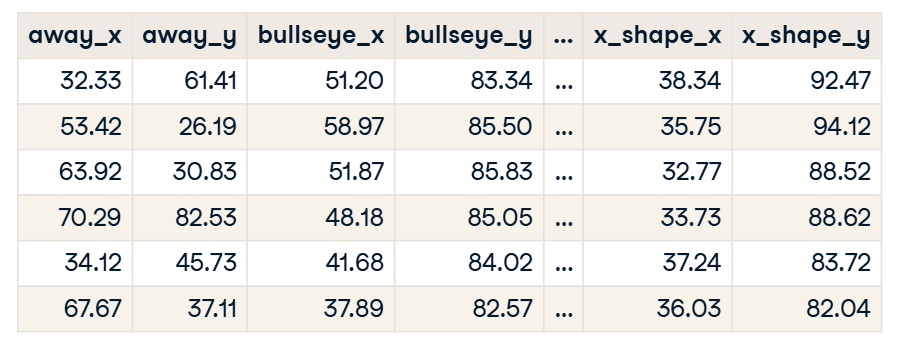
\includegraphics{../images/im1.png}
\end{frame}

\begin{frame}{The Datasaurus Dozen}
\phantomsection\label{the-datasaurus-dozen-2}
\begin{itemize}
\item
  Each dataset has two variables: the \textbf{x} and the \textbf{y}
  coordinates.
\item
  ``Variable'' is just statistics jargon for a column of data.
\end{itemize}
\end{frame}

\begin{frame}{Mean of x for each dataset}
\phantomsection\label{mean-of-x-for-each-dataset}
If you calculate the mean of the \textbf{x} values in each dataset, you
can see that it's more or less the same value.

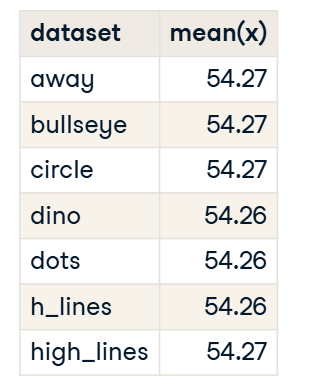
\includegraphics{../images/im2.png}
\end{frame}

\begin{frame}{Mean of x and y for each dataset}
\phantomsection\label{mean-of-x-and-y-for-each-dataset}
\begin{itemize}
\tightlist
\item
  It's the same situation for the means of the \textbf{y} coordinates.
\end{itemize}

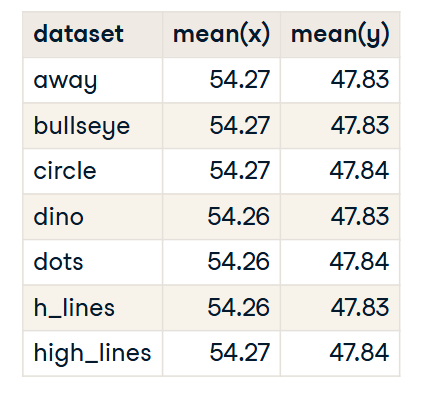
\includegraphics{../images/im3.png}
\end{frame}

\begin{frame}{Standard deviations for each dataset}
\phantomsection\label{standard-deviations-for-each-dataset}
\begin{itemize}
\item
  Similarly, we can look at the variation of the \textbf{x} and
  \textbf{y} values by calculating the standard deviation for each
  dataset.
\item
  Variation describes how spread out values are.
\item
  Each dataset has the same standard deviation for \textbf{x} and
  \textbf{y}.
\end{itemize}
\end{frame}

\begin{frame}{Standard deviations for each dataset}
\phantomsection\label{standard-deviations-for-each-dataset-1}
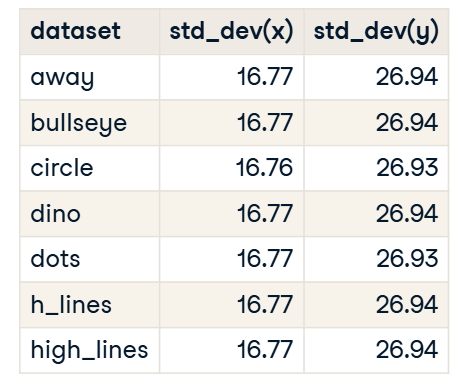
\includegraphics{../images/im4.png}
\end{frame}

\begin{frame}{Plotting dino}
\phantomsection\label{plotting-dino}
Here is a scatter plot of each dataset, and even a quick glance shows
what the calculations failed to.

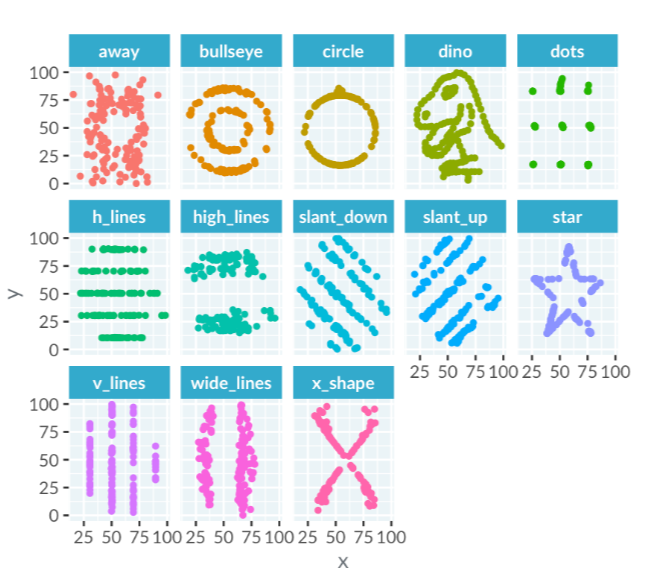
\includegraphics{../images/im5.png}
\end{frame}

\begin{frame}{Plotting dino}
\phantomsection\label{plotting-dino-1}
\begin{itemize}
\item
  That is, every dataset is completely different.
\item
  Until you physically look at the datasets, it's hard to tell that you
  have lines and circles and a star and a dinosaur.
\item
  The datasets are artificial, but I hope this example has convinced you
  of the importance of plotting your datasets.
\end{itemize}
\end{frame}

\begin{frame}{Continuous and categorical variables}
\phantomsection\label{continuous-and-categorical-variables}
\begin{itemize}
\item
  Before diving deeper into plotting, it's important to acknowledge that
  there are different types of data.
\item
  Choosing a type of plot depends on whether your variables are
  \textbf{continuous} or \textbf{categorical}.
\end{itemize}
\end{frame}

\begin{frame}{Continuous and categorical variables}
\phantomsection\label{continuous-and-categorical-variables-1}
\begin{itemize}
\tightlist
\item
  \textbf{Continuous: usually numbers}
\end{itemize}

heights, temperatures, revenues

You can do arithmetic on continuous variables, like adding two
temperatures together.
\end{frame}

\begin{frame}{Continuous and categorical variables}
\phantomsection\label{continuous-and-categorical-variables-2}
\begin{itemize}
\tightlist
\item
  \textbf{Categorical: usually text}
\end{itemize}

eye color, country, industry
\end{frame}

\begin{frame}{Continuous and categorical variables}
\phantomsection\label{continuous-and-categorical-variables-3}
Some things can either be \textbf{continuous} or \textbf{categorical}.

\begin{itemize}
\item
  \textbf{Age} is a number, so by default it's a \textbf{continuous}
  variable.
\item
  \textbf{age groups} like 25 to 30 are \textbf{categories}.
\end{itemize}
\end{frame}

\begin{frame}{Let's practice!}
\phantomsection\label{lets-practice}
It's time for your first set of exercises!
\end{frame}

\begin{frame}{Exercise 1 : Bitcoin price by date}
\phantomsection\label{exercise-1-bitcoin-price-by-date}
\begin{itemize}
\item
  To get an insight from a dataset, you can calculate summary statistics
  or run statistical models, but often it's easier to draw a plot.
\item
  In this exercise, you can see the price of the Bitcoin cryptocurrency
  from the start of 2016 to the start of 2020.
\item
  Look at the Bitcoin prices on January the first each year. Which year
  began with the highest Bitcoin price?
\end{itemize}
\end{frame}

\begin{frame}{Exercise 1 : Bitcoin price by date}
\phantomsection\label{exercise-1-bitcoin-price-by-date-1}
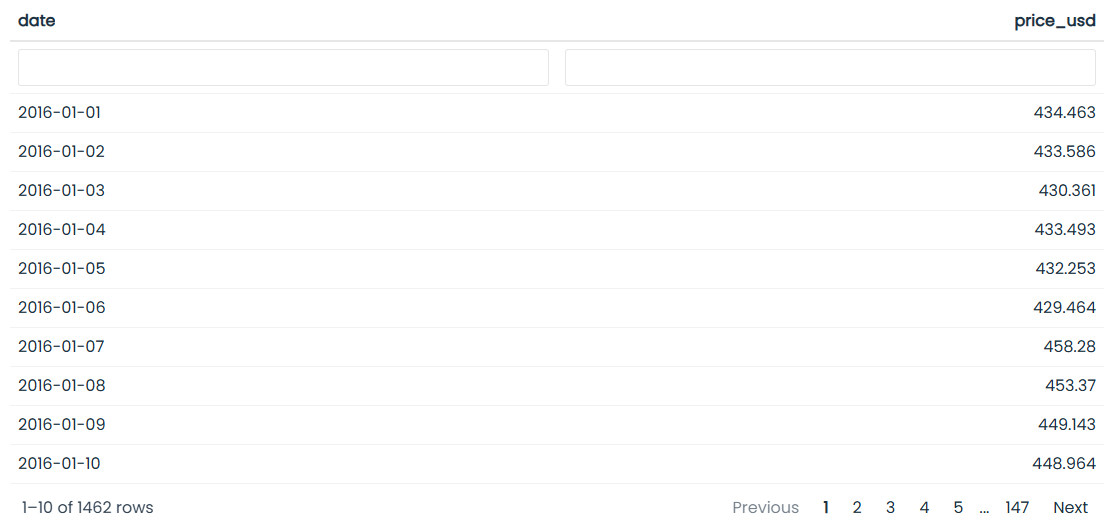
\includegraphics{../images/ex1_1.png}

You can filter and sort the data in the table, but it will be easier to
solve if you see results in a plot.
\end{frame}

\begin{frame}{Exercise 1 : Bitcoin price by date}
\phantomsection\label{exercise-1-bitcoin-price-by-date-2}
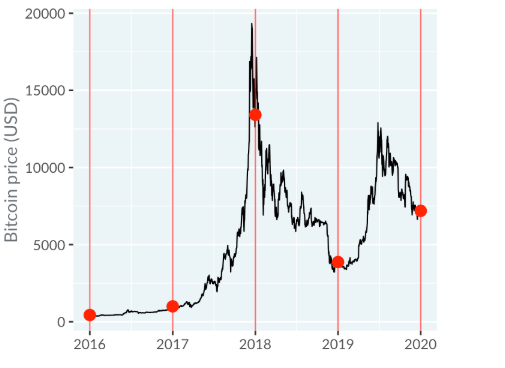
\includegraphics{../images/ex1_2.png}
\end{frame}

\begin{frame}{Exercise 2 : Continuous vs.~categorical variables}
\phantomsection\label{exercise-2-continuous-vs.-categorical-variables}
Was the exam passed or failed?
\end{frame}

\begin{frame}{Exercise 2 : Continuous vs.~categorical variables}
\phantomsection\label{exercise-2-continuous-vs.-categorical-variables-1}
Categorical
\end{frame}

\begin{frame}{Exercise 2 : Continuous vs.~categorical variables}
\phantomsection\label{exercise-2-continuous-vs.-categorical-variables-2}
Population of towns in Albania
\end{frame}

\begin{frame}{Exercise 2 : Continuous vs.~categorical variables}
\phantomsection\label{exercise-2-continuous-vs.-categorical-variables-3}
Continuous
\end{frame}

\begin{frame}{Exercise 2 : Continuous vs.~categorical variables}
\phantomsection\label{exercise-2-continuous-vs.-categorical-variables-4}
Job title of employees
\end{frame}

\begin{frame}{Exercise 2 : Continuous vs.~categorical variables}
\phantomsection\label{exercise-2-continuous-vs.-categorical-variables-5}
Categorical
\end{frame}

\begin{frame}{Exercise 2 : Continuous vs.~categorical variables}
\phantomsection\label{exercise-2-continuous-vs.-categorical-variables-6}
Salary of employees
\end{frame}

\begin{frame}{Exercise 2 : Continuous vs.~categorical variables}
\phantomsection\label{exercise-2-continuous-vs.-categorical-variables-7}
Continuous
\end{frame}

\begin{frame}{Exercise 2 : Continuous vs.~categorical variables}
\phantomsection\label{exercise-2-continuous-vs.-categorical-variables-8}
Provinces of towns in Albania
\end{frame}

\begin{frame}{Exercise 2 : Continuous vs.~categorical variables}
\phantomsection\label{exercise-2-continuous-vs.-categorical-variables-9}
Categorical
\end{frame}

\begin{frame}{Exercise 2 : Continuous vs.~categorical variables}
\phantomsection\label{exercise-2-continuous-vs.-categorical-variables-10}
Mass of products
\end{frame}

\begin{frame}{Exercise 2 : Continuous vs.~categorical variables}
\phantomsection\label{exercise-2-continuous-vs.-categorical-variables-11}
Continuous
\end{frame}

\begin{frame}{Histograms}
\phantomsection\label{histograms}
Let's explore histograms.
\end{frame}

\begin{frame}{When should you use a histogram?}
\phantomsection\label{when-should-you-use-a-histogram}
\begin{itemize}
\item
  Histograms are a type of plot that takes one continuous variable as
  its input.
\item
  It allows you to answer questions about the shape of that variable's
  distribution.
\item
  For example, you might want to know the lowest and highest values, and
  which values are most common.
\end{itemize}
\end{frame}

\begin{frame}{Kings and Queens of England \& Britain}
\phantomsection\label{kings-and-queens-of-england-britain}
Here's a dataset on the kings and queens of England, and more recently
Britain.

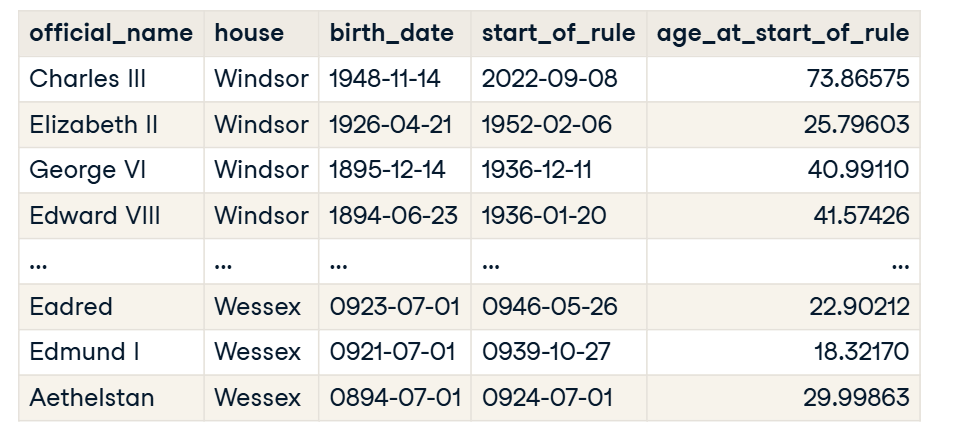
\includegraphics{../images/im6.png}
\end{frame}

\begin{frame}{Kings and Queens of England \& Britain}
\phantomsection\label{kings-and-queens-of-england-britain-1}
\begin{itemize}
\item
  It stretches from the current monarch back in time to the first king
  of England, Aethelstan.
\item
  Let's take a look at the distribution of the ages when they ascended
  to the throne.
\end{itemize}
\end{frame}

\begin{frame}{Histogram of age at start of rule}
\phantomsection\label{histogram-of-age-at-start-of-rule}
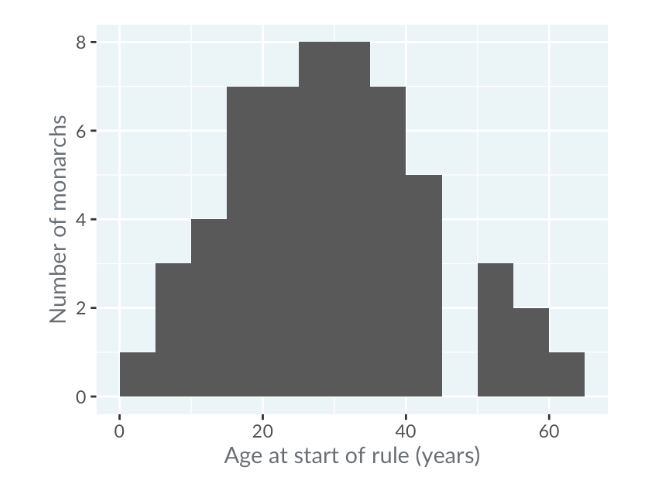
\includegraphics{../images/im7.png}
\end{frame}

\begin{frame}{Histogram of age at start of rule}
\phantomsection\label{histogram-of-age-at-start-of-rule-1}
\begin{itemize}
\item
  The x-axis is the variable that we are interested in - the
  \textbf{ages}.
\item
  These ages are grouped into ``bins'', that is, intervals.
\end{itemize}
\end{frame}

\begin{frame}{Histogram of age at start of rule}
\phantomsection\label{histogram-of-age-at-start-of-rule-2}
\begin{itemize}
\item
  In this case, the bins are zero to five years, five to ten years, and
  so on up to sixty to sixty five years.
\item
  The y-axis is the count of monarchs who began ruling when they were in
  each age bin.
\item
  For example, four monarchs began ruling when they were between ten and
  fifteen years old.
\item
  Straight away, you can see that there have been no monarchs who
  started ruling when they were between the ages of forty five and
  fifty.
\end{itemize}
\end{frame}

\begin{frame}{Choosing binwidth: 1 year}
\phantomsection\label{choosing-binwidth-1-year}
The appearance of a histogram is strongly influenced by the choice of
binwidth.

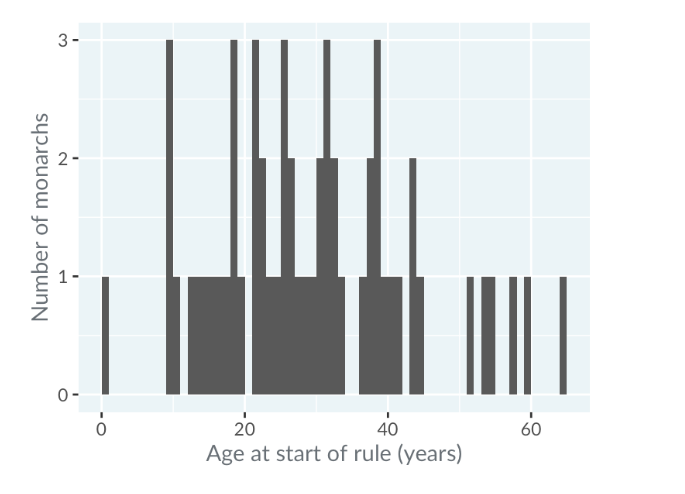
\includegraphics{../images/im8.png}
\end{frame}

\begin{frame}{Choosing binwidth: 1 year}
\phantomsection\label{choosing-binwidth-1-year-1}
\begin{itemize}
\item
  This is the same histogram as before, but with the binwidth changed
  from five years to one year.
\item
  It's difficult to get much insight into the distribution, because the
  counts are very noisy.
\item
  Choosing a binwidth that is too wide also causes problems.
\end{itemize}
\end{frame}

\begin{frame}{Choosing binwidth: 25 years}
\phantomsection\label{choosing-binwidth-25-years}
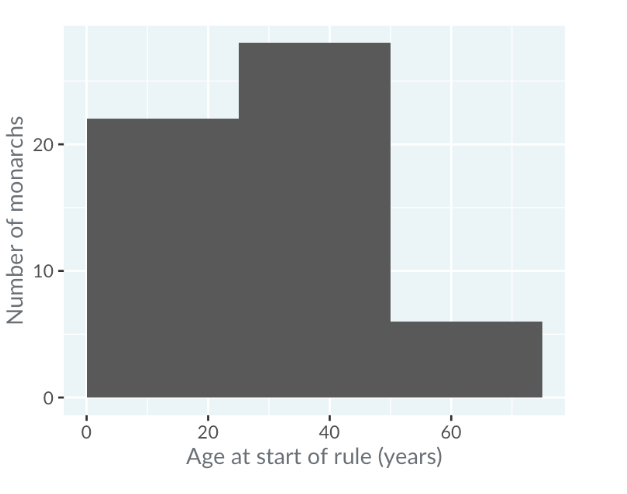
\includegraphics{../images/im9.png}
\end{frame}

\begin{frame}{Choosing binwidth: 25 years}
\phantomsection\label{choosing-binwidth-25-years-1}
\begin{itemize}
\item
  By changing the binwidth to twenty five years, you don't see any
  detail in the distribution, and again it is hard to get much insight.
\item
  In general, it is difficult to know the best binwidth before you draw
  the plot, so you'll need to experiment with several values.
\end{itemize}
\end{frame}

\begin{frame}{Modality: how many peaks?}
\phantomsection\label{modality-how-many-peaks}
\begin{itemize}
\item
  When interpreting histograms, the first thing to look at is the
  \textbf{modality} of the distribution.
\item
  That is, how many peaks there are.
\end{itemize}
\end{frame}

\begin{frame}{Modality: how many peaks?}
\phantomsection\label{modality-how-many-peaks-1}
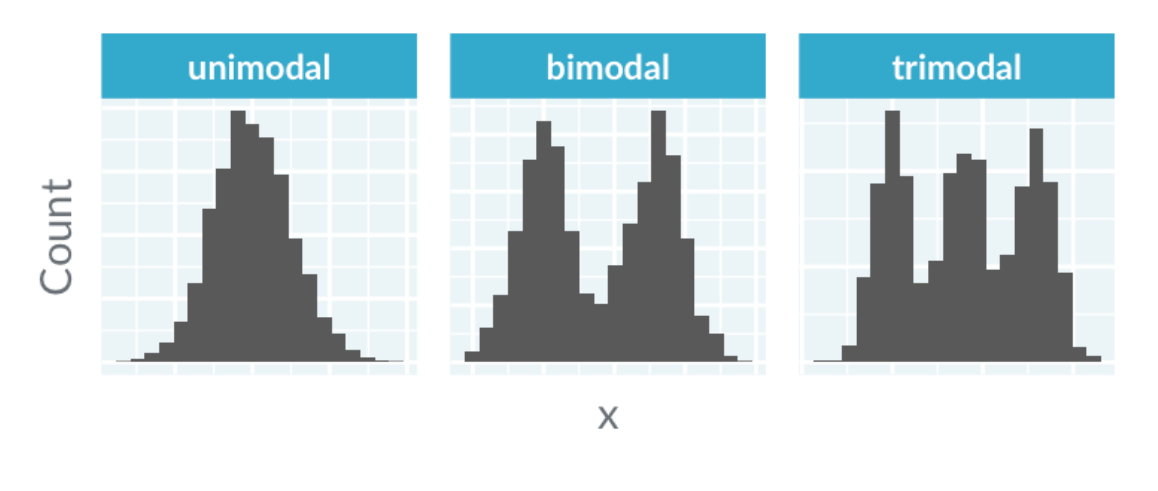
\includegraphics{../images/im10.png}
\end{frame}

\begin{frame}{Modality: how many peaks?}
\phantomsection\label{modality-how-many-peaks-2}
\begin{itemize}
\item
  A distribution with one peak is called \textbf{unimodal}
\item
  A distribution with two peaks is called \textbf{bimodal}, and so on.
\end{itemize}
\end{frame}

\begin{frame}{Modality: how many peaks?}
\phantomsection\label{modality-how-many-peaks-3}
Here, the distribution of ages is unimodal because there is one peak
from twenty five to thirty five years.

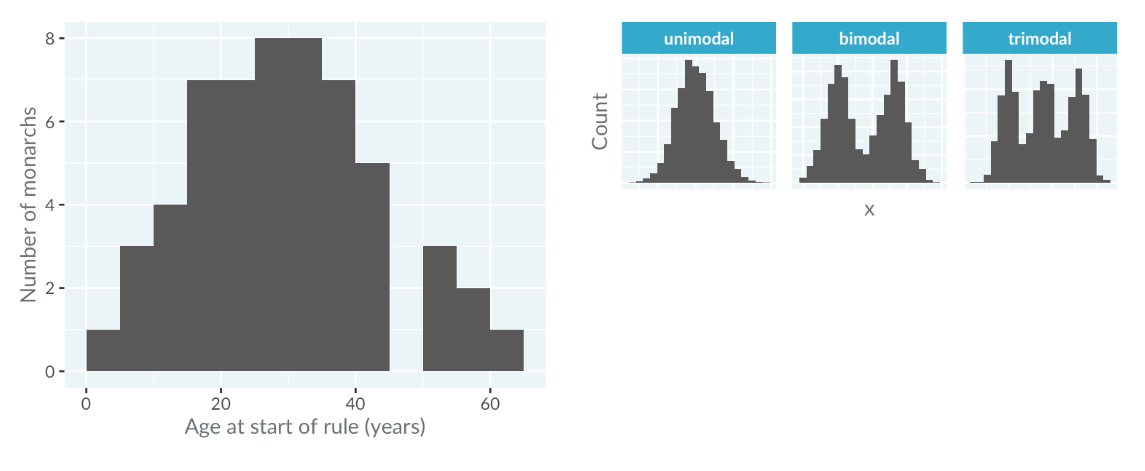
\includegraphics{../images/im11.png}
\end{frame}

\begin{frame}{Skewness: is it symmetric?}
\phantomsection\label{skewness-is-it-symmetric}
\begin{itemize}
\item
  The second thing to look at is the skewness of the distribution.
\item
  That's statistical jargon for whether or not it is symmetric.
\end{itemize}
\end{frame}

\begin{frame}{Skewness: is it symmetric?}
\phantomsection\label{skewness-is-it-symmetric-1}
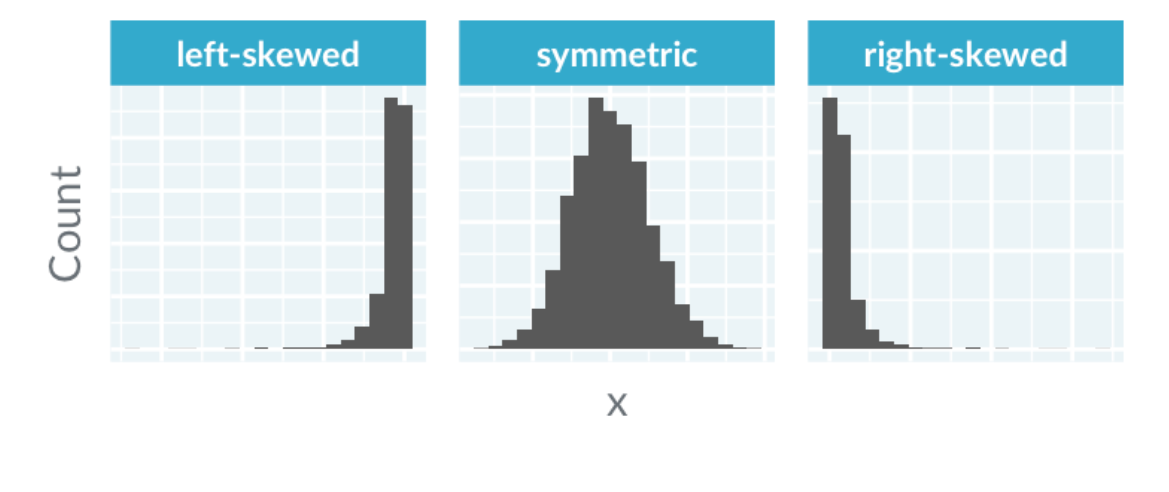
\includegraphics{../images/im12.png}
\end{frame}

\begin{frame}{Skewness: is it symmetric?}
\phantomsection\label{skewness-is-it-symmetric-2}
\begin{itemize}
\item
  A \textbf{left-skewed distribution} has outliers, that is, the extreme
  values, on the \textbf{left}
\item
  A \textbf{right-skewed distribution} has outliers on the
  \textbf{right}.
\end{itemize}
\end{frame}

\begin{frame}{Skewness: is it symmetric?}
\phantomsection\label{skewness-is-it-symmetric-3}
Here, the distribution is more or less symmetric.

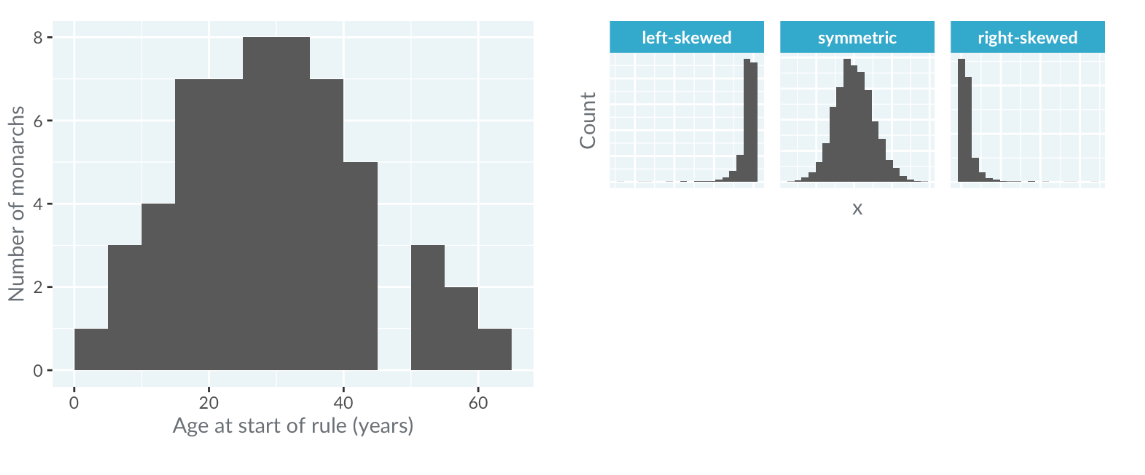
\includegraphics{../images/im13.png}
\end{frame}

\begin{frame}{Kurtosis: how many extreme values?}
\phantomsection\label{kurtosis-how-many-extreme-values}
\begin{itemize}
\tightlist
\item
  One more advanced thing you can look at is the \textbf{kurtosis} of
  the distribution, which affects the number of outliers.
\end{itemize}

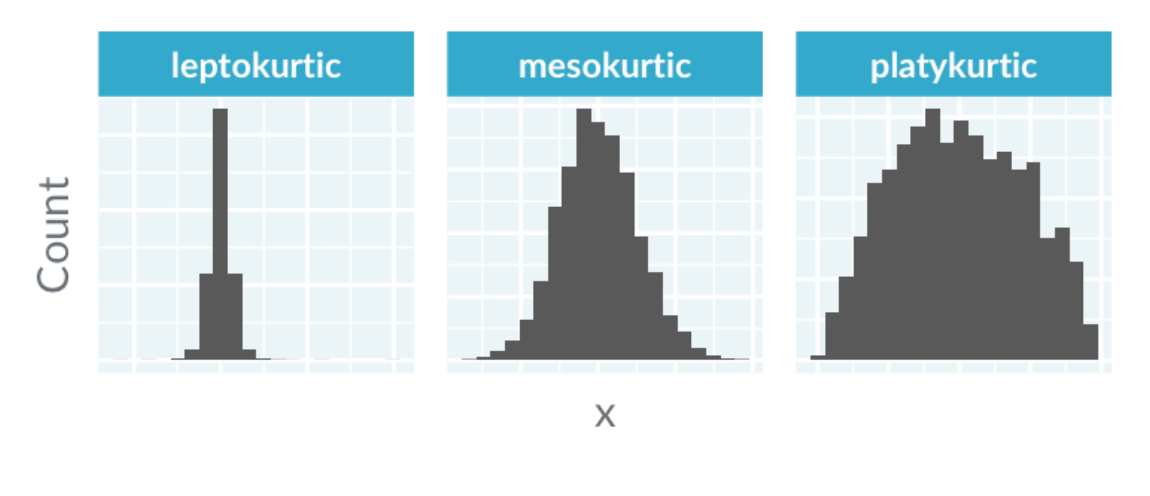
\includegraphics{../images/im14.png}
\end{frame}

\begin{frame}{Kurtosis: how many extreme values?}
\phantomsection\label{kurtosis-how-many-extreme-values-1}
\begin{itemize}
\item
  A \textbf{mesokurtic} distribution is something that looks like the
  bell curve from a normal distribution.
\item
  A \textbf{leptokurtic} distribution has a narrow peak and lots of
  extreme values. Leptokurtic distributions are important in finance,
  because weird stuff happens in stock markets more often than the
  normal distribution would predict.
\item
  A \textbf{platykurtic} distribution has a broad peak and few extreme
  values.
\end{itemize}
\end{frame}

\begin{frame}{Kurtosis: how many extreme values?}
\phantomsection\label{kurtosis-how-many-extreme-values-2}
Here, the distribution of ages is slightly platykurtic.

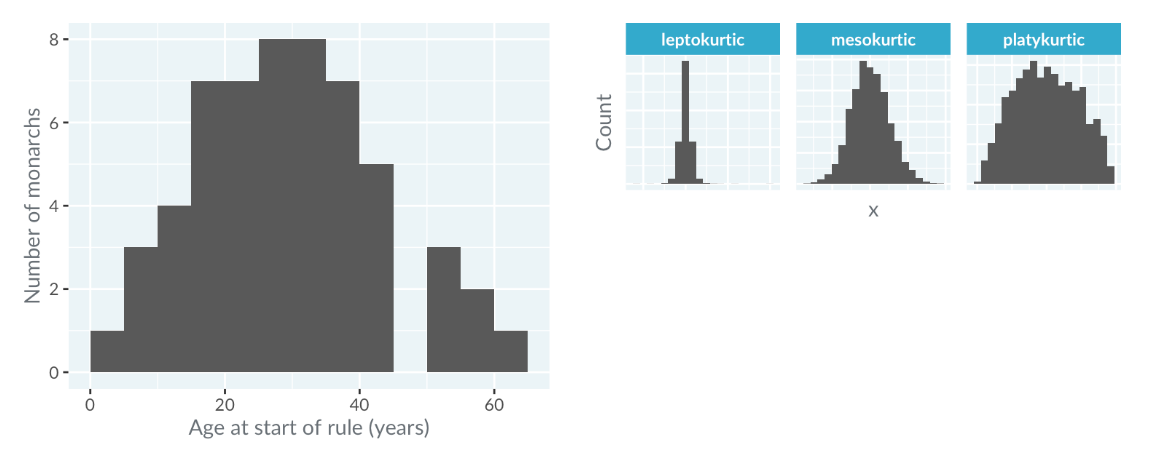
\includegraphics{../images/im15.png}
\end{frame}

\begin{frame}{Practice: Interpreting histograms}
\phantomsection\label{practice-interpreting-histograms}
Here is a histogram of salaries for various jobs in Australia. Each row
of the dataset is the average salary for that job, so the counts are
counts of jobs.

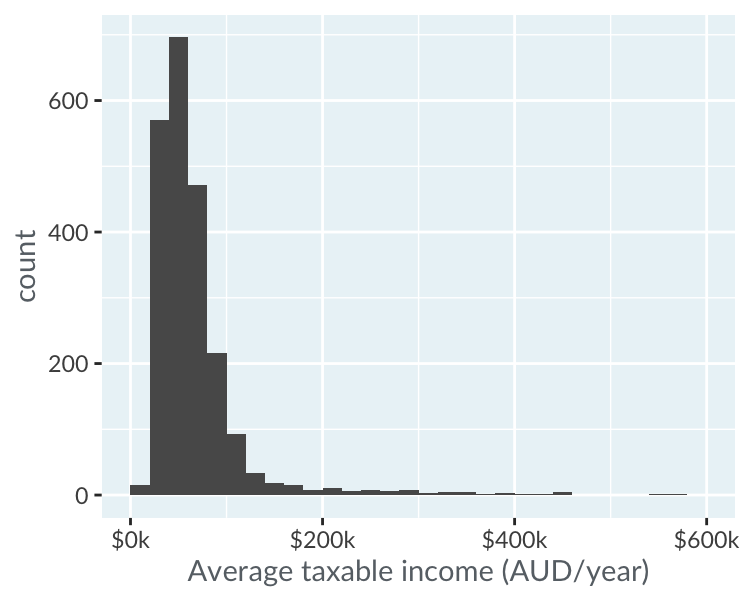
\includegraphics{../images/im16.png}
\end{frame}

\begin{frame}{Practice: Interpreting histograms}
\phantomsection\label{practice-interpreting-histograms-1}
TRUE or FALSE?

\emph{The most popular salary bracket is 40k to 60k}
\end{frame}

\begin{frame}{Practice: Interpreting histograms}
\phantomsection\label{practice-interpreting-histograms-2}
TRUE
\end{frame}

\begin{frame}{Practice: Interpreting histograms}
\phantomsection\label{practice-interpreting-histograms-3}
TRUE or FALSE?

\emph{The histogram is unimodal}
\end{frame}

\begin{frame}{Practice: Interpreting histograms}
\phantomsection\label{practice-interpreting-histograms-4}
TRUE
\end{frame}

\begin{frame}{Practice: Interpreting histograms}
\phantomsection\label{practice-interpreting-histograms-5}
TRUE or FALSE?

\emph{The histogram is right-skewed}
\end{frame}

\begin{frame}{Practice: Interpreting histograms}
\phantomsection\label{practice-interpreting-histograms-6}
TRUE
\end{frame}

\begin{frame}{Practice: Interpreting histograms}
\phantomsection\label{practice-interpreting-histograms-7}
TRUE or FALSE?

\emph{The most popular salary bracket is 560k to 580k}
\end{frame}

\begin{frame}{Practice: Interpreting histograms}
\phantomsection\label{practice-interpreting-histograms-8}
FALSE
\end{frame}

\begin{frame}{Practice: Interpreting histograms}
\phantomsection\label{practice-interpreting-histograms-9}
TRUE or FALSE?

\emph{The histogram is bimodal}
\end{frame}

\begin{frame}{Practice: Interpreting histograms}
\phantomsection\label{practice-interpreting-histograms-10}
FALSE
\end{frame}

\begin{frame}{Practice: Interpreting histograms}
\phantomsection\label{practice-interpreting-histograms-11}
TRUE or FALSE?

\emph{The histogram is left-skewed}
\end{frame}

\begin{frame}{Practice: Interpreting histograms}
\phantomsection\label{practice-interpreting-histograms-12}
FALSE
\end{frame}

\begin{frame}{Box plots}
\phantomsection\label{box-plots}
Individual histograms are great, but there is a problem if you want to
draw lots of them.
\end{frame}

\begin{frame}{You can't just color in histograms}
\phantomsection\label{you-cant-just-color-in-histograms}
\begin{itemize}
\item
  Let's revisit the kings and queens dataset.
\item
  Suppose we want to see the distribution of ages for each royal house.
\end{itemize}
\end{frame}

\begin{frame}{You can't just color in histograms}
\phantomsection\label{you-cant-just-color-in-histograms-1}
A naive solution might be to draw the same histogram, but using
different colors for each house. Sadly, this is a horrible muddled mess.

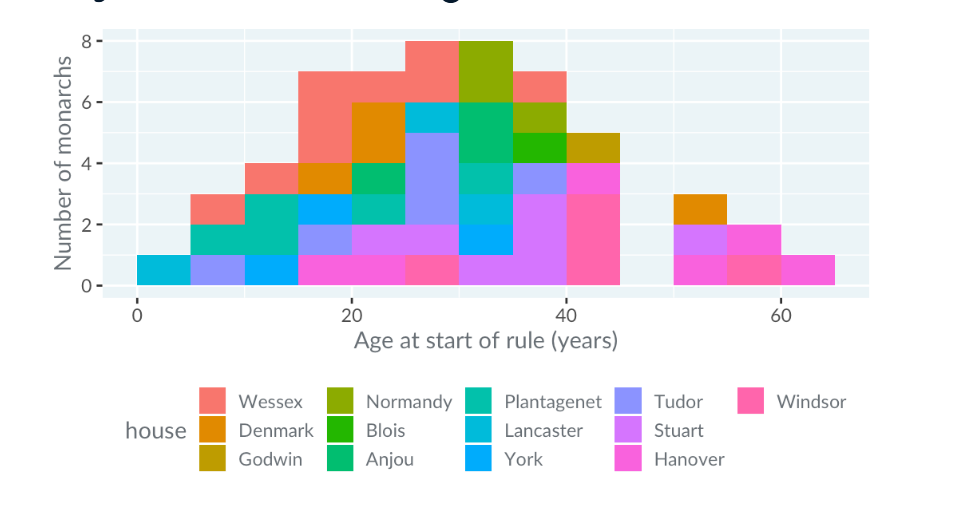
\includegraphics{../images/im17.png}
\end{frame}

\begin{frame}{Draw each histogram in its own panel}
\phantomsection\label{draw-each-histogram-in-its-own-panel}
\begin{itemize}
\tightlist
\item
  In many cases, the only sensible way to draw lots of histograms is to
  draw them in their own panel.
\end{itemize}

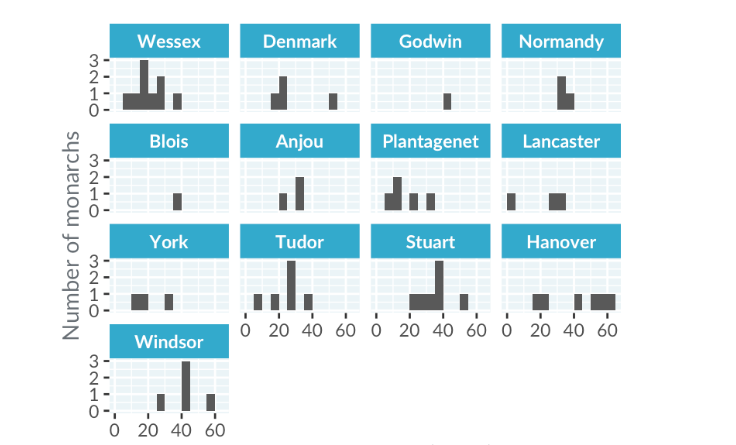
\includegraphics{../images/im18.png}
\end{frame}

\begin{frame}{Draw each histogram in its own panel}
\phantomsection\label{draw-each-histogram-in-its-own-panel-1}
\begin{itemize}
\item
  This approach still has problems.
\item
  It's quite easy to compare distributions for panels that are in the
  same column.
\end{itemize}
\end{frame}

\begin{frame}{Draw each histogram in its own panel}
\phantomsection\label{draw-each-histogram-in-its-own-panel-2}
You can see that monarchs from the Wessex family were typically much
younger when they began ruling than those from the Windsor family, since
you can look down the column and see that the Wessex distribution is to
the left of Windsor's.

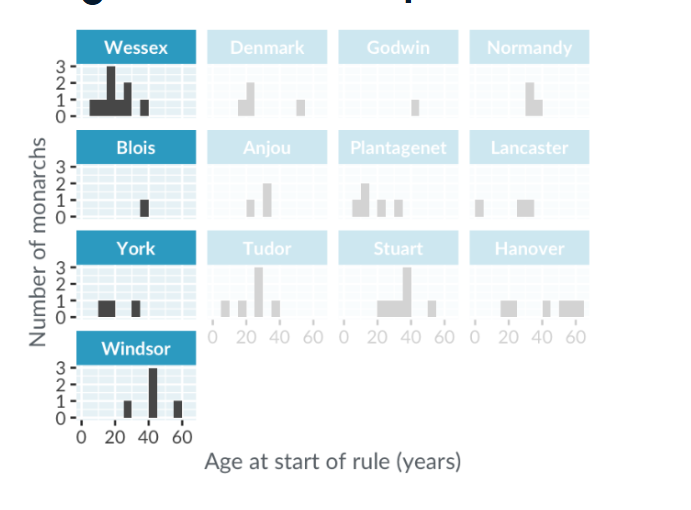
\includegraphics{../images/im19.png}
\end{frame}

\begin{frame}{Draw each histogram in its own panel}
\phantomsection\label{draw-each-histogram-in-its-own-panel-3}
By contrast, it's harder to compare distributions between panels that
are in different columns.
\end{frame}

\begin{frame}{Draw each histogram in its own panel}
\phantomsection\label{draw-each-histogram-in-its-own-panel-4}
To compare the ages of monarchs in the rival York and Lancaster houses,
you have to do a lot of looking back and forth and staring at numbers on
the x-axis, which isn't ideal.

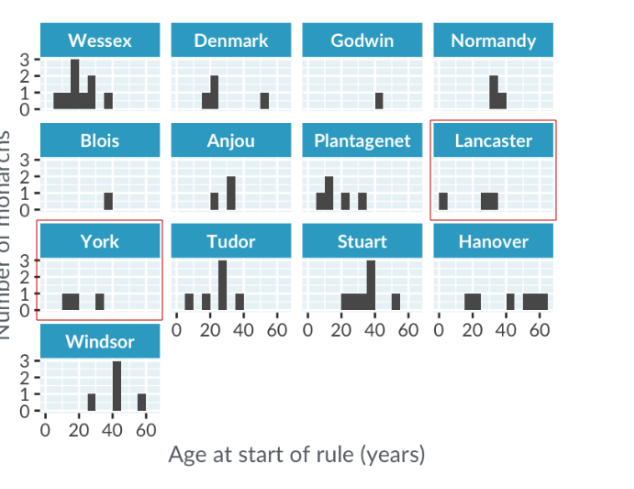
\includegraphics{../images/im20.png}
\end{frame}

\begin{frame}{Draw each histogram in its own panel}
\phantomsection\label{draw-each-histogram-in-its-own-panel-5}
\begin{itemize}
\tightlist
\item
  You could align all the panels in a single column, but that often
  means running out of space.
\end{itemize}
\end{frame}

\begin{frame}{Draw each histogram in its own panel}
\phantomsection\label{draw-each-histogram-in-its-own-panel-6}
Here, the text on the plot is almost unreadable. Fortunately, box plots
can solve our problems.

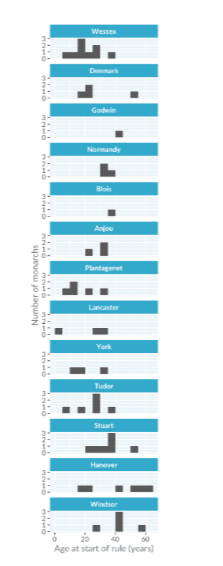
\includegraphics{../images/im21.png}
\end{frame}

\begin{frame}{When should you use a box plot?}
\phantomsection\label{when-should-you-use-a-box-plot}
\begin{itemize}
\item
  Box plots split a \textbf{continuous} variable - like \textbf{age} -
  by a \textbf{categorical} variable - like \textbf{royal house}
\item
  This allows us to compare the resulting distributions in a
  space-efficient way.
\end{itemize}
\end{frame}

\begin{frame}{Histogram vs.~box plot}
\phantomsection\label{histogram-vs.-box-plot}
Here's a comparison of the histogram you saw before with a box plot.

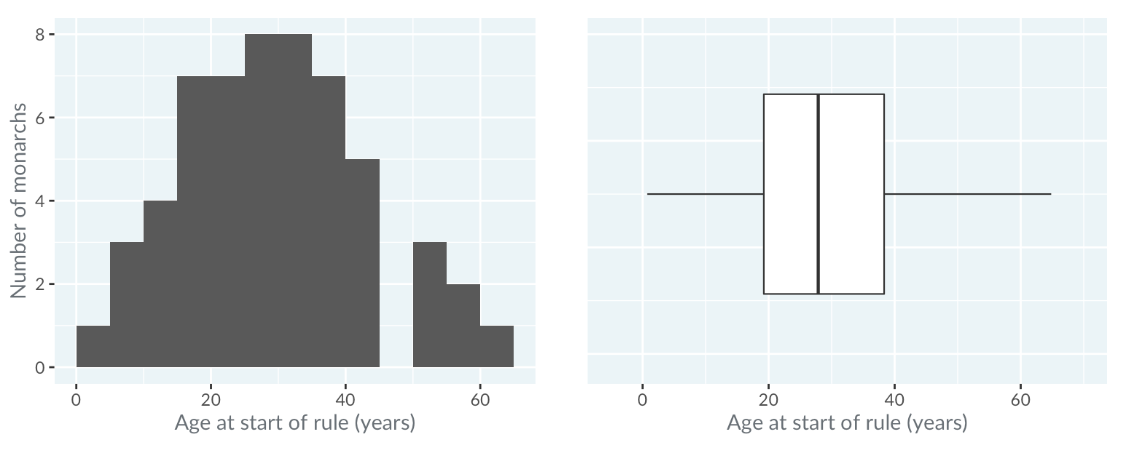
\includegraphics{../images/im22.png}
\end{frame}

\begin{frame}{Histogram vs.~box plot: mid-line}
\phantomsection\label{histogram-vs.-box-plot-mid-line}
The line in the middle shows the median of the distribution.

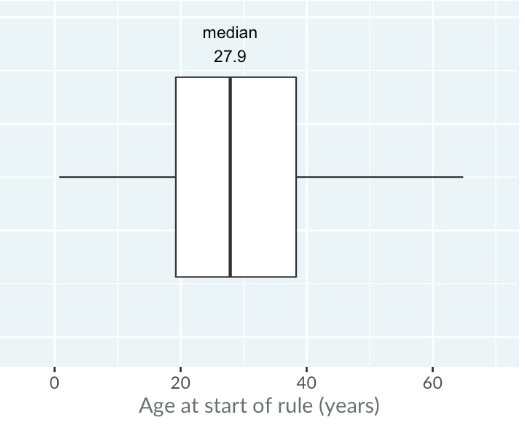
\includegraphics{../images/im24.png}

That is, half the monarchs started ruling before this age, and half
after this age.
\end{frame}

\begin{frame}{Histograms vs.~box plot: the box}
\phantomsection\label{histograms-vs.-box-plot-the-box}
The box in the box plot extends from the lower quartile to the upper
quartile.

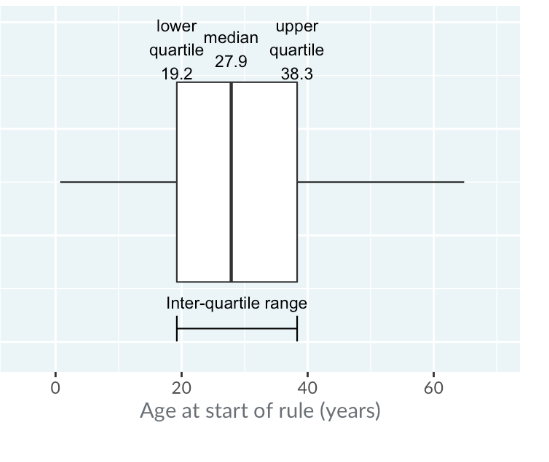
\includegraphics{../images/im25.png}
\end{frame}

\begin{frame}{Histograms vs.~box plot: the box}
\phantomsection\label{histograms-vs.-box-plot-the-box-1}
\begin{itemize}
\item
  The lower quartile is the point where one quarter of the values are
  below it.
\item
  That is, one quarter of the monarchs started ruling before this age,
  and three quarters after it.
\end{itemize}
\end{frame}

\begin{frame}{Histograms vs.~box plot: the box}
\phantomsection\label{histograms-vs.-box-plot-the-box-2}
\begin{itemize}
\item
  Likewise, the upper quartile is the age where three quarters of the
  monarchs started ruling below this age.
\item
  The difference between the upper quartile and the lower quartile is
  called the inter-quartile range.
\end{itemize}
\end{frame}

\begin{frame}{Histograms vs.~box plots: the whiskers}
\phantomsection\label{histograms-vs.-box-plots-the-whiskers}
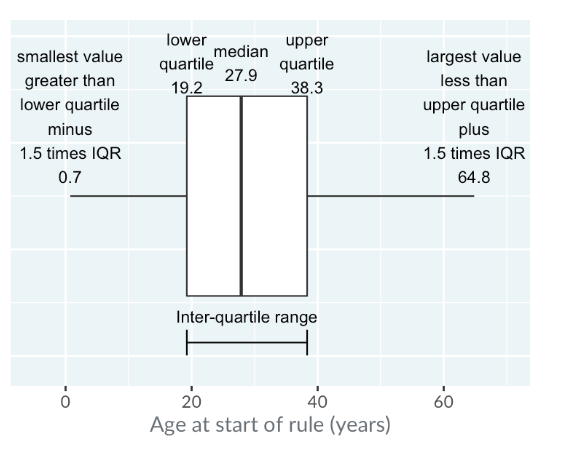
\includegraphics{../images/im27.png}
\end{frame}

\begin{frame}{Histograms vs.~box plots: the whiskers}
\phantomsection\label{histograms-vs.-box-plots-the-whiskers-1}
\begin{itemize}
\item
  The horizontal lines, known as ``whiskers'', have a more complicated
  definition.
\item
  Each bar extends to one and a half times the interquartile range, but
  then they are limited to reaching actual data points.
\item
  The technical definition is shown in the slide, but in practice, you
  can think of the whiskers as extending far enough that anything
  outside of them is an extreme value.
\end{itemize}
\end{frame}

\begin{frame}{Monarchs by house}
\phantomsection\label{monarchs-by-house}
As mentioned before, the power of box plots is that you can compare many
distributions at once.

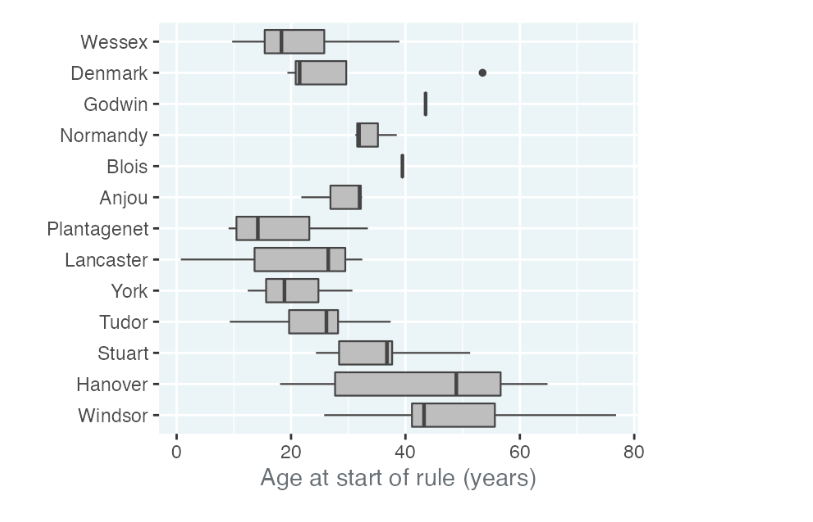
\includegraphics{../images/im28.png}
\end{frame}

\begin{frame}{Monarchs by house}
\phantomsection\label{monarchs-by-house-1}
\begin{itemize}
\tightlist
\item
  Here, the royal houses are ordered from oldest at the top to newest at
  the bottom.
\end{itemize}

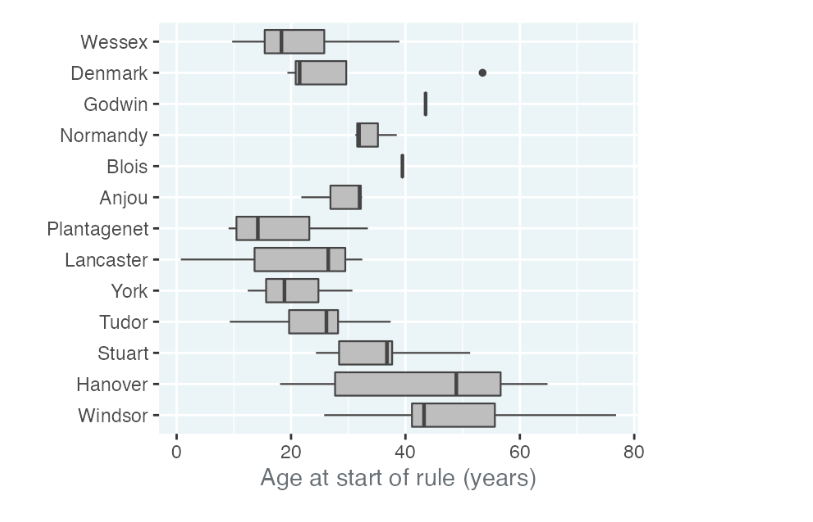
\includegraphics{../images/im28.png}

\begin{itemize}
\tightlist
\item
  A trend is visible: since the Plantagenets in the fourteenth century,
  the boxes gradually move right showing that the ages when new monarchs
  ascend to the throne have been increasing.
\end{itemize}
\end{frame}

\begin{frame}{Monarchs by house}
\phantomsection\label{monarchs-by-house-2}
\begin{itemize}
\tightlist
\item
  Godwin and Blois appear as a single line because there was only one
  king from each house.
\end{itemize}

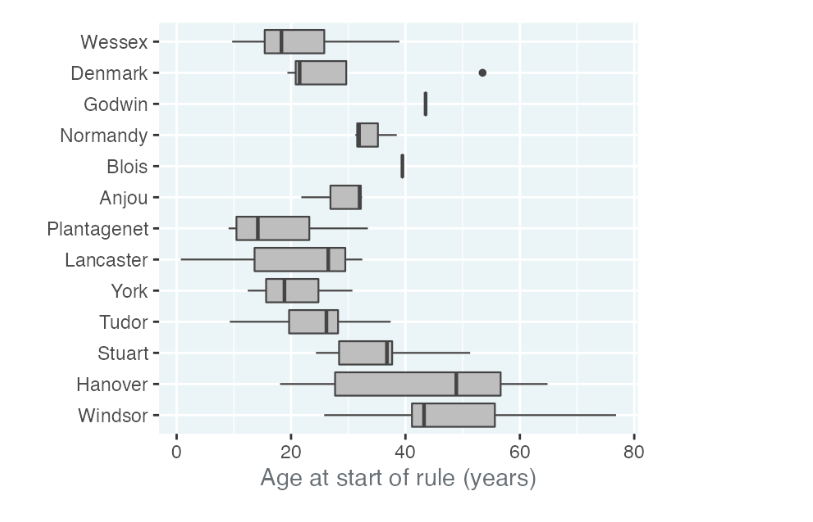
\includegraphics{../images/im28.png}

\begin{itemize}
\tightlist
\item
  The Anjou house only had three kings, and forms a box with one
  whisker, not two.
\end{itemize}
\end{frame}

\begin{frame}{Monarchs by house}
\phantomsection\label{monarchs-by-house-3}
\begin{itemize}
\tightlist
\item
  Notice that the box plot for the house of Denmark shows a point.
\end{itemize}

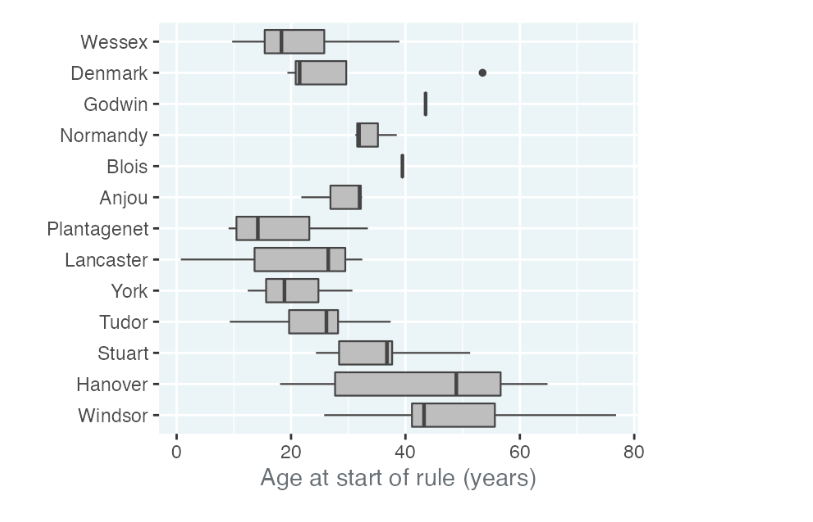
\includegraphics{../images/im28.png}

\begin{itemize}
\tightlist
\item
  Points are extreme values, that is, values that are outside the range
  of the whiskers. Denmark's right-most outlier is Sweyn who ascended at
  age 53, which was exceptionally high for the 11th century.
\end{itemize}
\end{frame}

\begin{frame}{Practice: Interpreting box plots}
\phantomsection\label{practice-interpreting-box-plots}
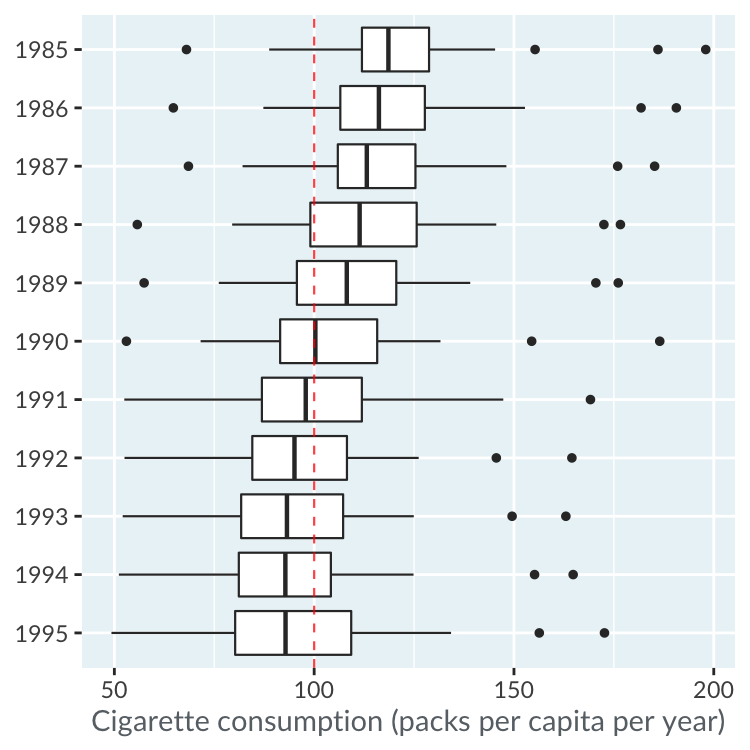
\includegraphics{../images/im29.png}

\begin{itemize}
\tightlist
\item
  Here are box plots of cigarette consumption per person in the USA from
  1985 to 1995 (Alaska and Hawaii are not included).
\end{itemize}
\end{frame}

\begin{frame}{Practice: Interpreting box plots}
\phantomsection\label{practice-interpreting-box-plots-1}
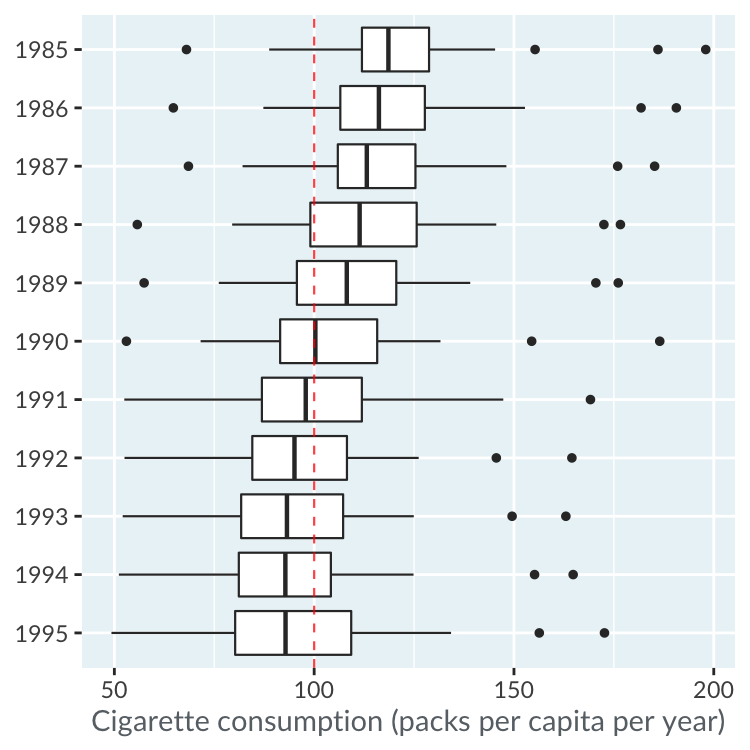
\includegraphics{../images/im29.png}

\begin{itemize}
\tightlist
\item
  Each observation in the dataset is the average number of packets of
  cigarette smoked per person in one state in one year.
\end{itemize}
\end{frame}

\begin{frame}{Practice: Interpreting box plots}
\phantomsection\label{practice-interpreting-box-plots-2}
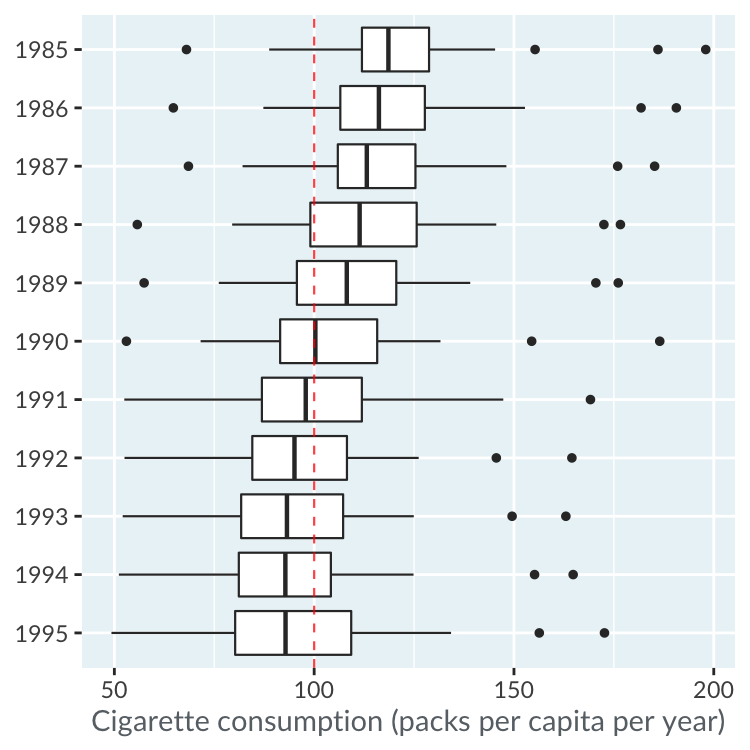
\includegraphics{../images/im29.png}

\begin{itemize}
\tightlist
\item
  Thus each box plot represents the distribution of 48 data points
  (because there are 48 US states included in the dataset).
\end{itemize}
\end{frame}

\begin{frame}{Practice: Interpreting box plots}
\phantomsection\label{practice-interpreting-box-plots-3}
TRUE or FALSE?

\emph{The lower quartile number of packets of cigarettes smoked per
capita decreased every year from 1985 to 1995.}
\end{frame}

\begin{frame}{Practice: Interpreting histograms}
\phantomsection\label{practice-interpreting-histograms-13}
TRUE
\end{frame}

\begin{frame}{Practice: Interpreting histograms}
\phantomsection\label{practice-interpreting-histograms-14}
TRUE or FALSE?

\emph{The upper quartile number of packets of cigarettes smoked per
capita decreased every year from 1985 to 1995.}
\end{frame}

\begin{frame}{Practice: Interpreting histograms}
\phantomsection\label{practice-interpreting-histograms-15}
FALSE
\end{frame}

\begin{frame}{Practice: Interpreting histograms}
\phantomsection\label{practice-interpreting-histograms-16}
TRUE or FALSE?

\emph{The median number of packets of cigarettes smoked per capita was
below 100 from 1991 onwards.}
\end{frame}

\begin{frame}{Practice: Interpreting histograms}
\phantomsection\label{practice-interpreting-histograms-17}
TRUE
\end{frame}

\begin{frame}{Practice: Interpreting histograms}
\phantomsection\label{practice-interpreting-histograms-18}
TRUE or FALSE?

\emph{The inter-quartile range of the number of packets of cigarettes
smoked per capita was smallest in 1992.}
\end{frame}

\begin{frame}{Practice: Interpreting histograms}
\phantomsection\label{practice-interpreting-histograms-19}
FALSE
\end{frame}

\begin{frame}{Practice: Interpreting histograms}
\phantomsection\label{practice-interpreting-histograms-20}
TRUE or FALSE?

\emph{The inter-quartile range of the number of packets of cigarettes
smoked per capita decreased every year from 1985 to 1995.}
\end{frame}

\begin{frame}{Practice: Interpreting histograms}
\phantomsection\label{practice-interpreting-histograms-21}
FALSE
\end{frame}

\begin{frame}{Practice: Interpreting histograms}
\phantomsection\label{practice-interpreting-histograms-22}
TRUE or FALSE?

\emph{In 1990, three states were considered to have extreme values in
the number of packets of cigarettes smoked per capita.}
\end{frame}

\begin{frame}{Practice: Interpreting histograms}
\phantomsection\label{practice-interpreting-histograms-23}
TRUE
\end{frame}

\section{Visualizing two variables}\label{visualizing-two-variables}

\begin{frame}{Scatter plots}
\phantomsection\label{scatter-plots}
\begin{itemize}
\item
  Far now we focused on visualizing one variable.
\item
  Now, we'll move on to two variables, beginning with scatter plots.
\end{itemize}
\end{frame}

\begin{frame}{When should you use a scatter plot?}
\phantomsection\label{when-should-you-use-a-scatter-plot}
\begin{itemize}
\item
  When you have two continuous variables, and you want to know about
  their relationship.
\item
  For example, if one variable increases, does the other one increase
  too, or does it decrease?
\end{itemize}
\end{frame}

\begin{frame}{Los Angeles County home prices}
\phantomsection\label{los-angeles-county-home-prices}
\begin{itemize}
\tightlist
\item
  Here's a dataset on home prices in four cities in Los Angeles County
  in 2012.
\end{itemize}

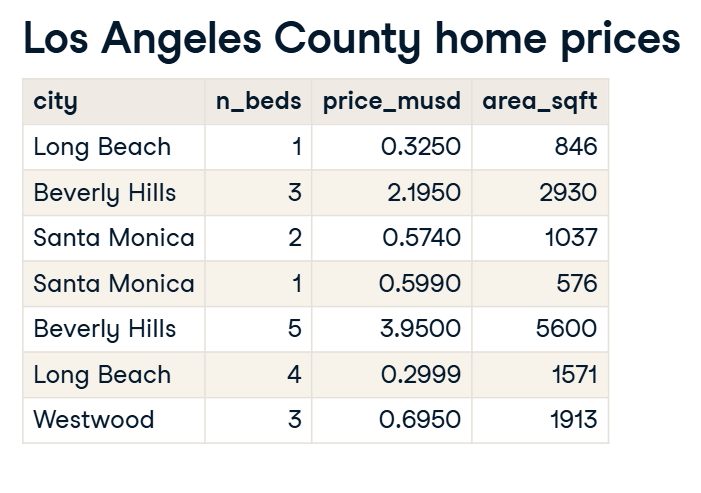
\includegraphics{../images/im30.png}
\end{frame}

\begin{frame}{Los Angeles County home prices}
\phantomsection\label{los-angeles-county-home-prices-1}
The dataset includes the number of bedrooms, the sale price in millions
of dollars, and the area in square feet.
\end{frame}

\begin{frame}{Prices vs.~area}
\phantomsection\label{prices-vs.-area}
Here's a scatter plot with the price on the y-axis and the area on the
x-axis.

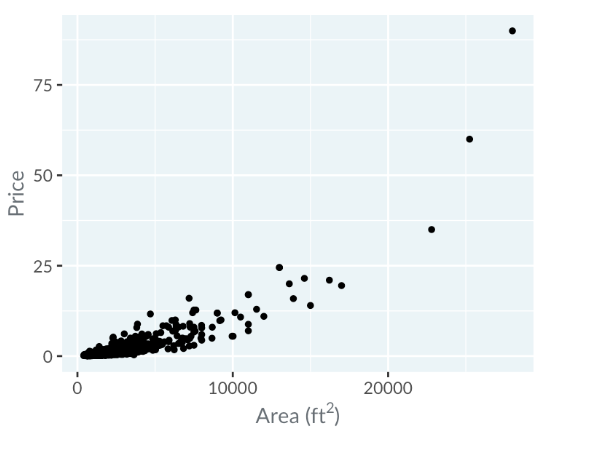
\includegraphics{../images/im31.png}
\end{frame}

\begin{frame}{Prices vs.~area}
\phantomsection\label{prices-vs.-area-1}
\begin{itemize}
\item
  We'd say it's a scatter plot of ``price versus area''.
\item
  It's OK, but all the points are clustered in the bottom left, making
  it hard to read.
\end{itemize}
\end{frame}

\begin{frame}{Prices vs.~area}
\phantomsection\label{prices-vs.-area-2}
Let's use a logarithmic scale for each axis.

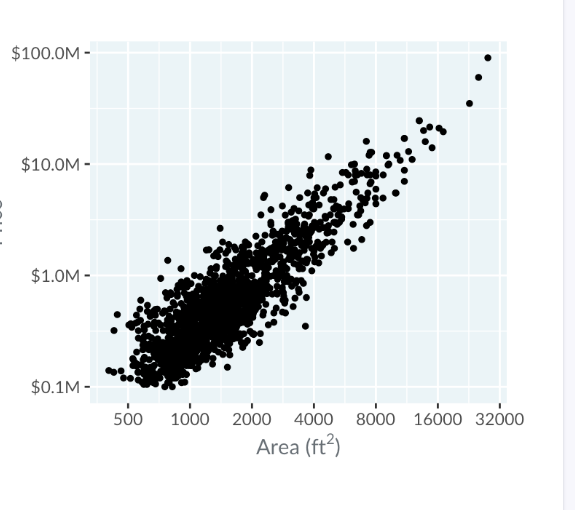
\includegraphics{../images/im32.png}
\end{frame}

\begin{frame}{Prices vs.~area}
\phantomsection\label{prices-vs.-area-3}
On the logarithmic plot, notice that moving right one grid line doubles
the area, or moving up one grid line multiples the price by a factor of
ten. Now the points are more evenly spread throughout the plot.

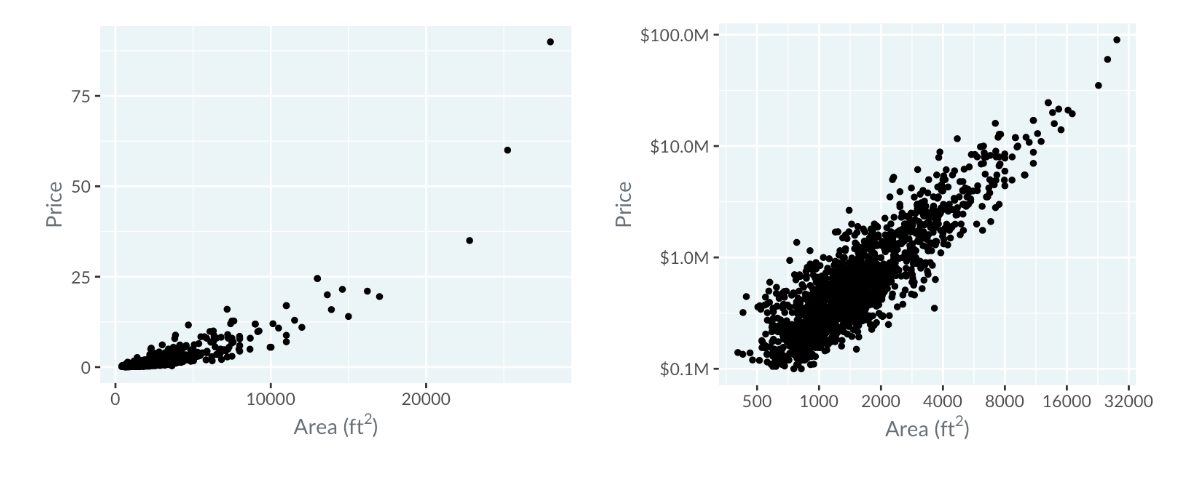
\includegraphics{../images/im33.png}
\end{frame}

\begin{frame}{Correlation}
\phantomsection\label{correlation}
\begin{itemize}
\item
  One important concept when interpreting scatter plots is the idea of
  correlation.
\item
  Roughly speaking, correlation is a measure of how well you can draw a
  straight line through the points.
\end{itemize}
\end{frame}

\begin{frame}{Correlation}
\phantomsection\label{correlation-1}
If that straight line goes upwards as you move to the right, it's called
a positive correlation.

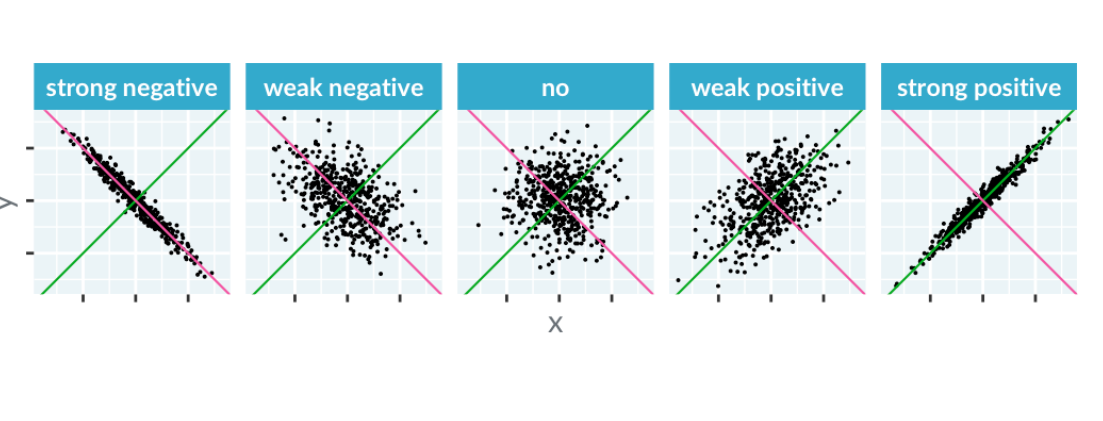
\includegraphics{../images/im34.png}
\end{frame}

\begin{frame}{Correlation}
\phantomsection\label{correlation-2}
If the line goes down as you go to the right, it's called negative
correlation.

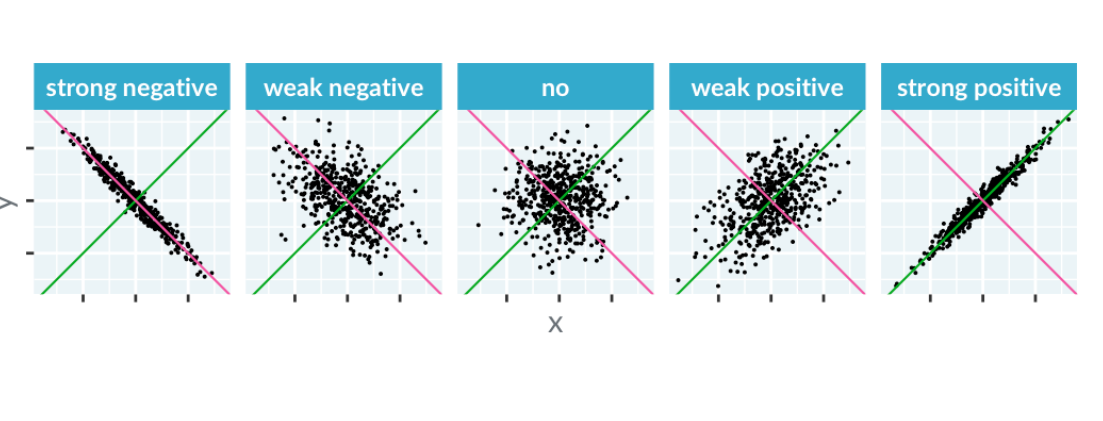
\includegraphics{../images/im34.png}
\end{frame}

\begin{frame}{Correlation}
\phantomsection\label{correlation-3}
Here are five theoretical datasets.

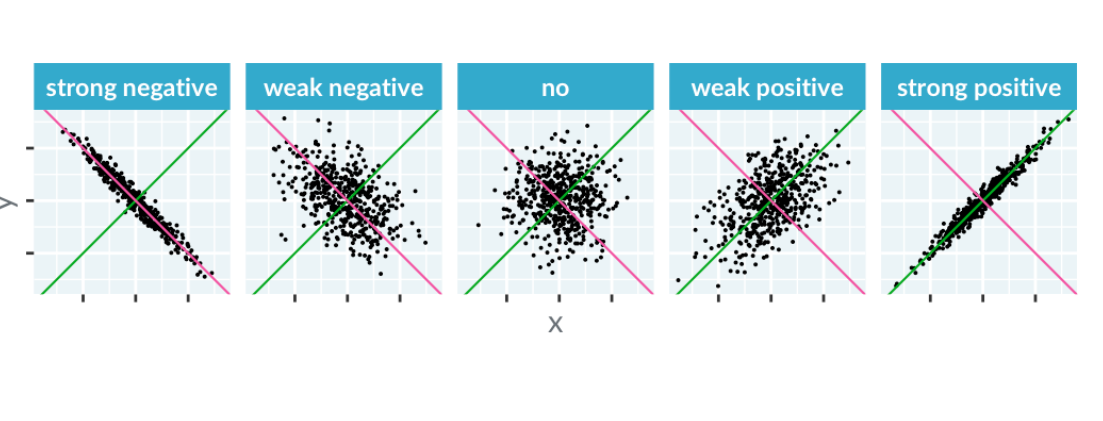
\includegraphics{../images/im34.png}
\end{frame}

\begin{frame}{Correlation}
\phantomsection\label{correlation-4}
The red line in each panel shows what perfect negative correlation would
look like.

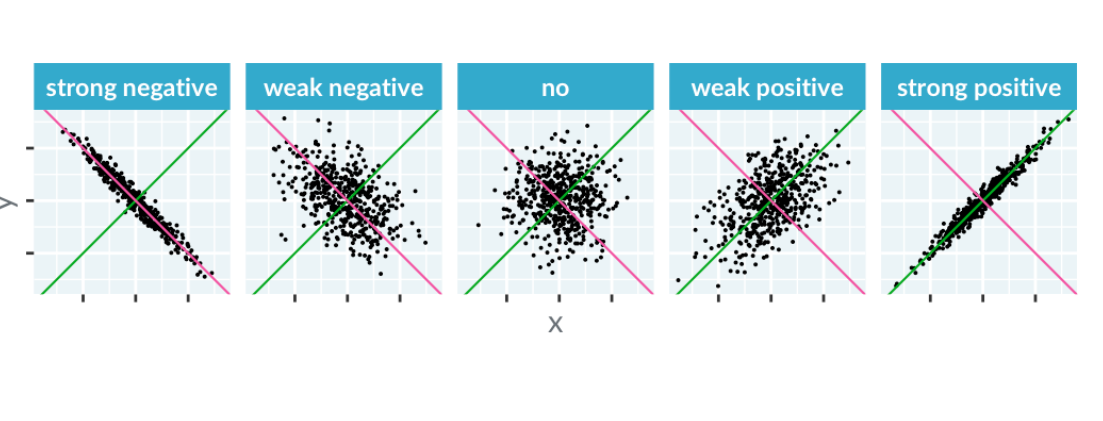
\includegraphics{../images/im34.png}
\end{frame}

\begin{frame}{Correlation}
\phantomsection\label{correlation-5}
The green lines show perfect positive correlation.

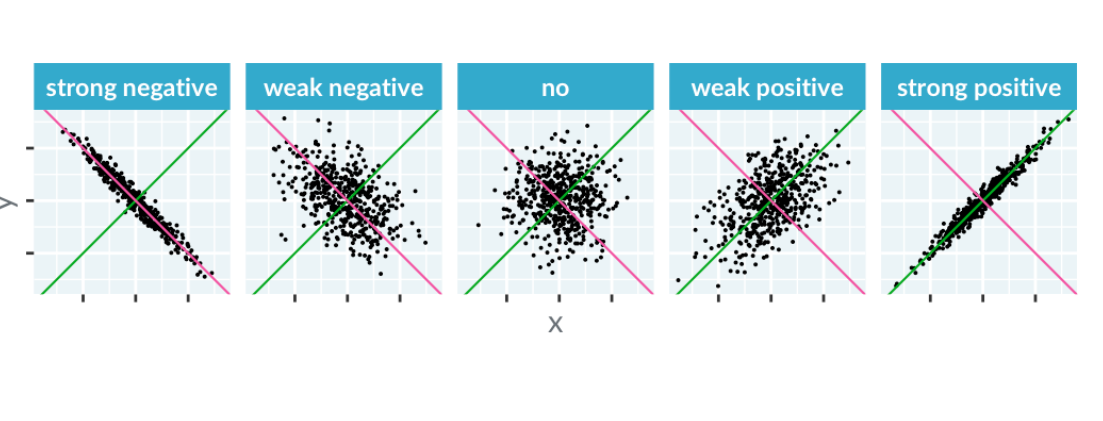
\includegraphics{../images/im34.png}
\end{frame}

\begin{frame}{Correlation}
\phantomsection\label{correlation-6}
In the left-most panel, you can see an example of strong negative
correlation.

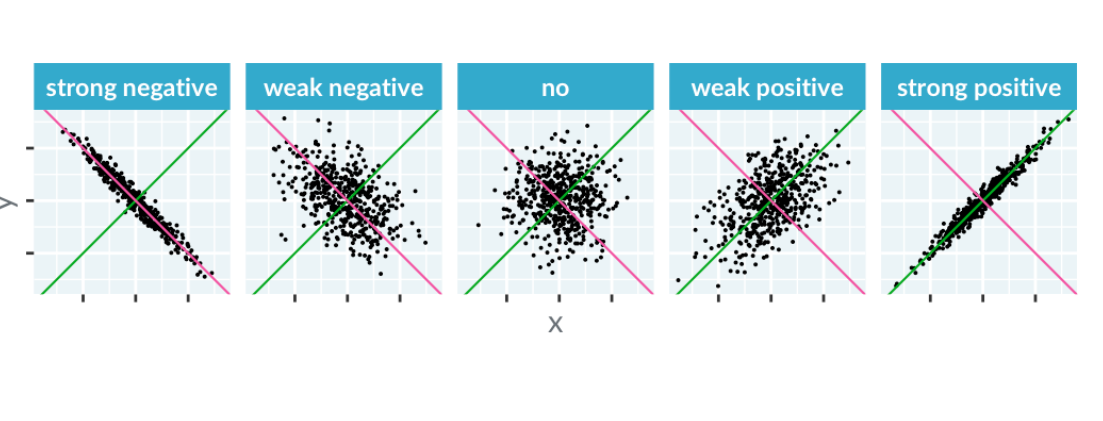
\includegraphics{../images/im34.png}
\end{frame}

\begin{frame}{Correlation}
\phantomsection\label{correlation-7}
In the left-most panel, you can see an example of strong negative
correlation.

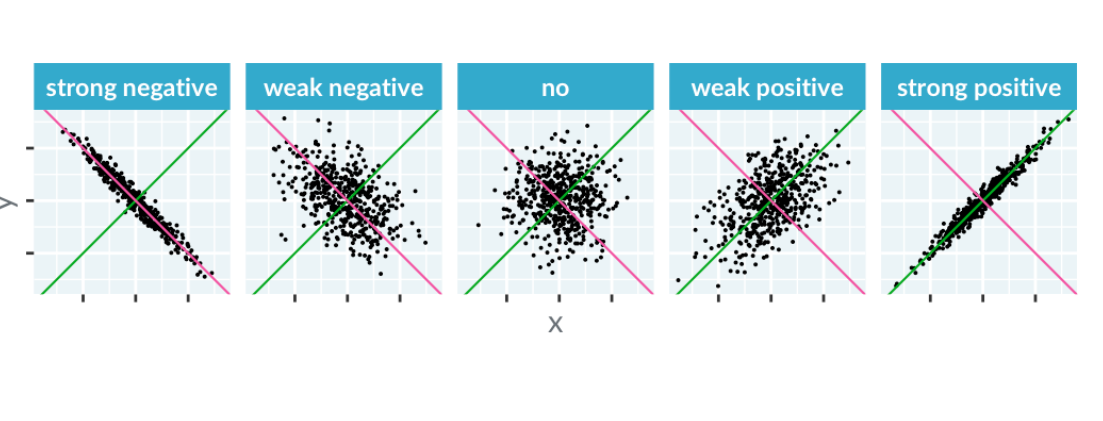
\includegraphics{../images/im34.png}
\end{frame}

\begin{frame}{Correlation}
\phantomsection\label{correlation-8}
In the left-most panel, you can see an example of strong negative
correlation. That means that as the x values increase, the y values
decrease.

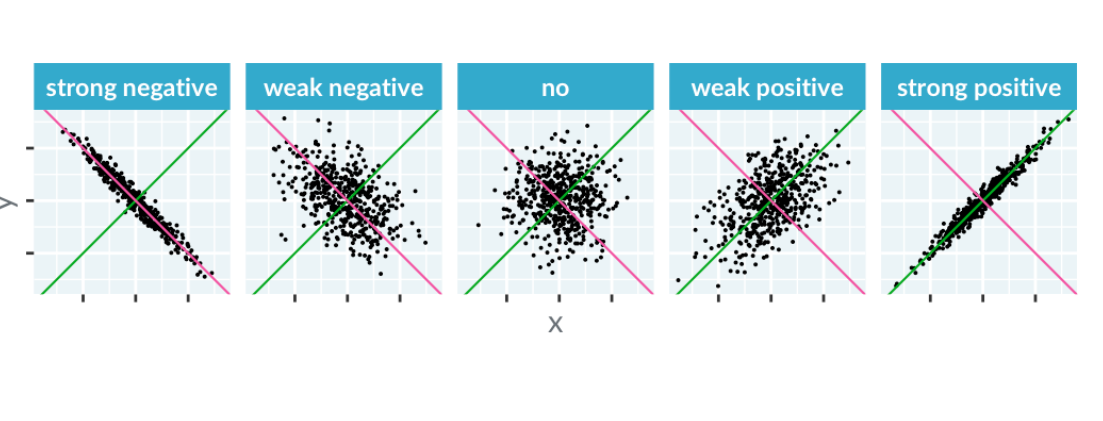
\includegraphics{../images/im34.png}
\end{frame}

\begin{frame}{Correlation}
\phantomsection\label{correlation-9}
In the right-most panel, you can see strong positive correlation,
meaning that as x increases, so does y.

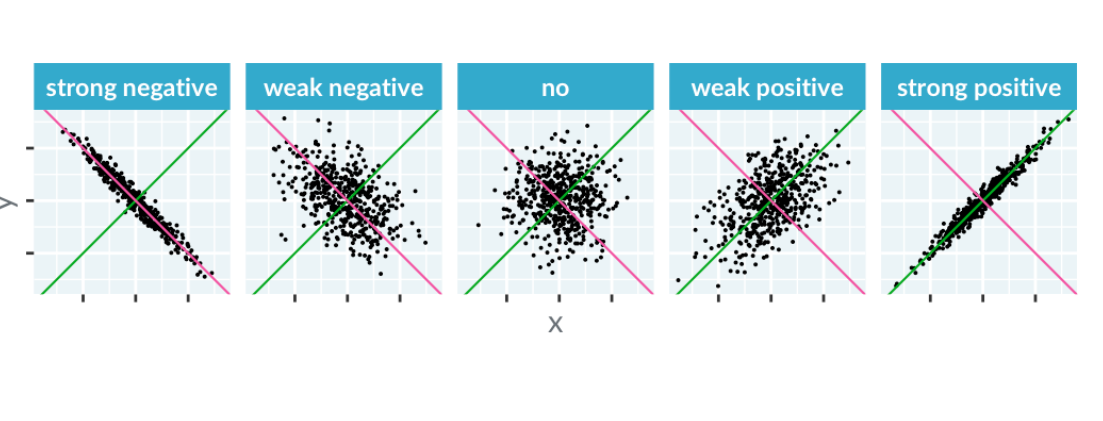
\includegraphics{../images/im34.png}
\end{frame}

\begin{frame}{Correlation}
\phantomsection\label{correlation-10}
The middle panels show intermediate states. In the third panel, showing
no correlation, the values of y are completely unrelated to the values
of x.

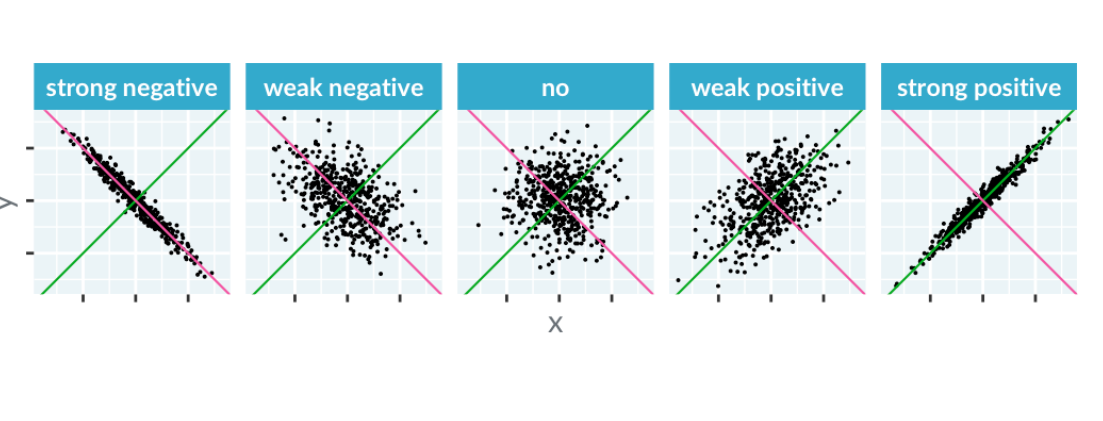
\includegraphics{../images/im34.png}
\end{frame}

\begin{frame}{Sometimes correlation isn't helpful}
\phantomsection\label{sometimes-correlation-isnt-helpful}
Here's the Datasaurus Dozen again.

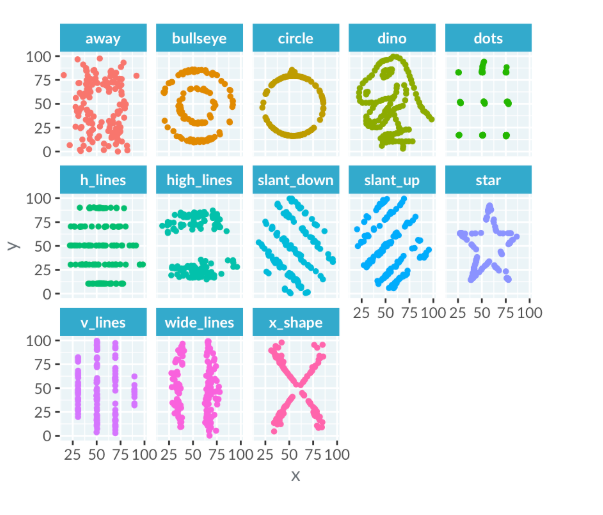
\includegraphics{../images/im35.png}
\end{frame}

\begin{frame}{Sometimes correlation isn't helpful}
\phantomsection\label{sometimes-correlation-isnt-helpful-1}
\begin{itemize}
\item
  Recall that each dataset had the same correlation, despite looking
  very different.
\item
  Correlation makes the most sense if there is a straight line
  relationship between the x and y values.
\end{itemize}
\end{frame}

\begin{frame}{Sometimes correlation isn't helpful}
\phantomsection\label{sometimes-correlation-isnt-helpful-2}
\begin{itemize}
\item
  If you have a more complicated shape, you'll need to be more creative
  in how you describe the relationship.
\item
  For example, ``x and y have a slight negative correlation'' is not as
  good a description as ``the plot looks like a dinosaur''.
\end{itemize}
\end{frame}

\begin{frame}{Adding trend lines}
\phantomsection\label{adding-trend-lines}
\begin{itemize}
\tightlist
\item
  Adding a straight line to a scatter plot is a great way to see you if
  you really do have a linear relationship between the x and y
  variables.
\end{itemize}

\includegraphics{../images/im36.png}
\end{frame}

\begin{frame}{Adding trend lines}
\phantomsection\label{adding-trend-lines-1}
\begin{itemize}
\tightlist
\item
  Here, with the logarithmic scales, the trend line has a close fit to
  the points, suggesting that as the logarithm of the area increases,
  you get a linear increase in the logarithm of the price.
\end{itemize}
\end{frame}

\begin{frame}{Adding smooth trend lines}
\phantomsection\label{adding-smooth-trend-lines}
\begin{itemize}
\tightlist
\item
  Sometimes a straight line might be a terrible fit.
\end{itemize}
\end{frame}

\begin{frame}{Adding smooth trend lines}
\phantomsection\label{adding-smooth-trend-lines-1}
Here, in the price versus area plot using a linear scale, the line
completely misses the more expensive homes.

\includegraphics{../images/im38.png}
\end{frame}

\begin{frame}{Adding smooth trend lines}
\phantomsection\label{adding-smooth-trend-lines-2}
\begin{itemize}
\tightlist
\item
  When a straight trend line is a poor fit, one alternative is to use a
  curve.
\end{itemize}

\includegraphics{../images/im39.png}

Having a curve like this can help you find a way to describe the
relationship. Here, by seeing the trend line curve upwards, you can say
``as area increases, the price increases faster than linearly''.
\end{frame}

\begin{frame}{Practice: Interpreting scatter plots}
\phantomsection\label{practice-interpreting-scatter-plots}
Scatter plots let you explore the relationship between two continuous
variables.
\end{frame}

\begin{frame}{Practice: Interpreting scatter plots}
\phantomsection\label{practice-interpreting-scatter-plots-1}
\includegraphics{../images/im40.png}

Here you can see a scatter plot of average life expectancy (on the
y-axis) versus average length of schooling (on the x-axis) for countries
around the world.
\end{frame}

\begin{frame}{Practice: Interpreting scatter plots}
\phantomsection\label{practice-interpreting-scatter-plots-2}
\begin{itemize}
\item
  Each point in the plot represents one country.
\item
  A straight trend line from a linear regression model is shown.
\end{itemize}
\end{frame}

\begin{frame}{Question 1: True or False?}
\phantomsection\label{question-1-true-or-false}
There is a positive correlation between the life expectancy and the
length of schooling.

\includegraphics{../images/im40.png}
\end{frame}

\begin{frame}{Answer to Question 1}
\phantomsection\label{answer-to-question-1}
\textbf{TRUE}
\end{frame}

\begin{frame}{Question 2: True or False?}
\phantomsection\label{question-2-true-or-false}
As the average length of schooling increases, the average life
expectancy typically increases too.

\includegraphics{../images/im40.png}
\end{frame}

\begin{frame}{Answer to Question 2}
\phantomsection\label{answer-to-question-2}
\textbf{TRUE}
\end{frame}

\begin{frame}{Question 3: True or False?}
\phantomsection\label{question-3-true-or-false}
Every country with an average life expectancy of less than 60 years has
an average length of schooling less than 7 years.

\includegraphics{../images/im40.png}
\end{frame}

\begin{frame}{Answer to Question 3}
\phantomsection\label{answer-to-question-3}
\textbf{TRUE}
\end{frame}

\begin{frame}{Question 4: True or False?}
\phantomsection\label{question-4-true-or-false}
If one country has a longer average length of schooling than another
country, that country will also have a greater average life expectancy.

\includegraphics{../images/im40.png}
\end{frame}

\begin{frame}{Answer to Question 4}
\phantomsection\label{answer-to-question-4}
\textbf{FALSE}
\end{frame}

\begin{frame}{Question 5: True or False?}
\phantomsection\label{question-5-true-or-false}
No countries have an average length of schooling less than 6 years and
an average life expectancy of more than 75 years.

\includegraphics{../images/im40.png}
\end{frame}

\begin{frame}{Answer to Question 5}
\phantomsection\label{answer-to-question-5}
\textbf{FALSE}
\end{frame}

\begin{frame}{Question 6: True or False?}
\phantomsection\label{question-6-true-or-false}
There is a negative correlation between the life expectancy and the
length of schooling.

\includegraphics{../images/im40.png}
\end{frame}

\begin{frame}{Answer to Question 6}
\phantomsection\label{answer-to-question-6}
\textbf{FALSE}
\end{frame}

\begin{frame}{Worldwide COVID-19 coronavirus cases}
\phantomsection\label{worldwide-covid-19-coronavirus-cases}
Here is a mildly terrifying scatter plot of the cumulative number of
cases of COVID-19 coronavirus throughout the world in early 2020.

\includegraphics{../images/im41.png}
\end{frame}

\begin{frame}{Worldwide COVID-19 coronavirus cases}
\phantomsection\label{worldwide-covid-19-coronavirus-cases-1}
\begin{itemize}
\item
  It's OK, but we can make a better plot.
\item
  Since the x-axis consists of dates, consecutive data points are
  connected.
\item
  That means that the plot is easier to understand if we connect those
  data points.
\item
  That is, using a line is preferable to points here.
\end{itemize}
\end{frame}

\begin{frame}{When Should You Use a Line Plot?}
\phantomsection\label{when-should-you-use-a-line-plot}
\begin{itemize}
\item
  Line plots are similar to scatter plots but connect consecutive data
  points to show trends.
\item
  Key requirements:

  \begin{itemize}
  \item
    You have two continuous variables.
  \item
    Consecutive observations are connected conceptually (e.g., dates or
    times).
  \end{itemize}
\item
  Example: Tracking COVID-19 cases over time.
\end{itemize}
\end{frame}

\begin{frame}{Comparing Multiple Lines}
\phantomsection\label{comparing-multiple-lines}
Line plots allow the comparison of multiple series within the same
graph.

\includegraphics{../images/im42.png}
\end{frame}

\begin{frame}{Comparing Multiple Lines}
\phantomsection\label{comparing-multiple-lines-1}
\begin{itemize}
\item
  Example:

  \begin{itemize}
  \item
    In February 2020, most COVID-19 cases were reported in
    \textbf{China}.
  \item
    By March, cases outside of China overtook the number in China.
  \end{itemize}
\item
  This provides a clear view of how trends differ across groups.
\end{itemize}
\end{frame}

\begin{frame}{Trend Lines}
\phantomsection\label{trend-lines}
\begin{itemize}
\tightlist
\item
  Trend lines show patterns in the data, such as linear relationships.
\end{itemize}

\includegraphics{../images/im43.png}
\end{frame}

\begin{frame}{Trend Lines}
\phantomsection\label{trend-lines-1}
\begin{itemize}
\item
  Example:

  \begin{itemize}
  \tightlist
  \item
    Data from March 2020 in China shows that the number of cases grew
    linearly after quarantine measures were implemented.
  \end{itemize}
\item
  Overlaying trend lines helps compare data behavior to theoretical
  models.
\end{itemize}
\end{frame}

\begin{frame}{Trend Lines with Logarithmic Scales}
\phantomsection\label{trend-lines-with-logarithmic-scales}
\begin{itemize}
\tightlist
\item
  Linear trend lines may not always fit the data.
\end{itemize}

\includegraphics{../images/im44.png}
\end{frame}

\begin{frame}{Trend Lines with Logarithmic Scales}
\phantomsection\label{trend-lines-with-logarithmic-scales-1}
\begin{itemize}
\item
  Example:

  \begin{itemize}
  \item
    Cases outside of China grew exponentially, making a linear trend
    line inappropriate.
  \item
    Applying a \textbf{logarithmic scale} to the y-axis reveals
    exponential growth clearly.
  \end{itemize}
\item
  Logarithmic scales are useful for rapid growth or varying orders of
  magnitude.
\end{itemize}
\end{frame}

\begin{frame}{Trend Lines with Logarithmic Scales}
\phantomsection\label{trend-lines-with-logarithmic-scales-2}
\includegraphics{../images/im45.png}
\end{frame}

\begin{frame}{Time on the X-Axis Doesn't Always Mean Line Plots}
\phantomsection\label{time-on-the-x-axis-doesnt-always-mean-line-plots}
\begin{itemize}
\tightlist
\item
  Just because the x-axis represents time, a \textbf{line plot} isn't
  always the best choice.
\end{itemize}

\includegraphics{../images/im46.png} \#\# Time on the X-Axis Doesn't
Always Mean Line Plots

\begin{itemize}
\item
  Example:

  \begin{itemize}
  \item
    A scatter plot of hip-hop song ratings (x-axis = date, y-axis =
    critic's score).
  \item
    Songs are independent, so connecting them with lines would be
    misleading.
  \end{itemize}
\item
  Always assess whether consecutive points are conceptually connected.
\end{itemize}
\end{frame}

\begin{frame}{Lines Aren't Always Necessary for Time}
\phantomsection\label{lines-arent-always-necessary-for-time}
\begin{itemize}
\item
  Example:

  \begin{itemize}
  \tightlist
  \item
    Plot of juvenile offenders in Switzerland (x-axis = time, y-axis =
    number of offenders).
  \end{itemize}
\end{itemize}

\includegraphics{../images/im47.png}
\end{frame}

\begin{frame}{Lines Aren't Always Necessary for Time}
\phantomsection\label{lines-arent-always-necessary-for-time-1}
Each line represents an age group.

\begin{itemize}
\item
  Problem:

  \begin{itemize}
  \tightlist
  \item
    The line plot may not provide clear insights.
  \end{itemize}
\end{itemize}
\end{frame}

\begin{frame}{Practice: Interpreting line plots}
\phantomsection\label{practice-interpreting-line-plots}
\begin{itemize}
\item
  Line plots are excellent for comparing two continuous variables, where
  consecutive observations are connected somehow.
\item
  A common type of line plot is to have dates or times on the x-axis,
  and a numeric quantity on the y-axis.
\end{itemize}
\end{frame}

\begin{frame}{Practice: Interpreting line plots}
\phantomsection\label{practice-interpreting-line-plots-1}
\begin{itemize}
\item
  In this case, ``consecutive observations'' means values on successive
  dates, like today and tomorrow.
\item
  By drawing multiple lines on the same plot, you can compare values.
\end{itemize}
\end{frame}

\begin{frame}{Practice: Interpreting line plots}
\phantomsection\label{practice-interpreting-line-plots-2}
The following line plot shows the percentage of households in the United
States that adopted each of four technologies (automobiles,
refrigerators, stoves, and vacuums) from 1930 to 1970.

\includegraphics{../images/im48.png}
\end{frame}

\begin{frame}{Question 1: True or False?}
\phantomsection\label{question-1-true-or-false-1}
After 1940, adoption of refrigerators was always higher than adoption of
stoves.

\includegraphics{../images/im48.png}
\end{frame}

\begin{frame}{Answer to Question 1}
\phantomsection\label{answer-to-question-1-1}
\textbf{TRUE}
\end{frame}

\begin{frame}{Question 2: True or False?}
\phantomsection\label{question-2-true-or-false-1}
In 1945, two out of the four technologies had lower adoption than in
1940.

\includegraphics{../images/im48.png}
\end{frame}

\begin{frame}{Answer to Question 2}
\phantomsection\label{answer-to-question-2-1}
\textbf{TRUE}
\end{frame}

\begin{frame}{Question 3: True or False?}
\phantomsection\label{question-3-true-or-false-1}
In 1930, adoption of automobiles was greater than 50\%.

\includegraphics{../images/im48.png}
\end{frame}

\begin{frame}{Answer to Question 3}
\phantomsection\label{answer-to-question-3-1}
\textbf{TRUE}
\end{frame}

\begin{frame}{Question 4: True or False?}
\phantomsection\label{question-4-true-or-false-1}
It took longer for refrigerators to go from 50\% adoption to 75\%
adoption than it took vacuums.

\includegraphics{../images/im48.png}
\end{frame}

\begin{frame}{Answer to Question 4}
\phantomsection\label{answer-to-question-4-1}
\textbf{FALSE}
\end{frame}

\begin{frame}{Question 5: True or False?}
\phantomsection\label{question-5-true-or-false-1}
In 1940, adoption of stoves was greater than adoption of automobiles.

\includegraphics{../images/im48.png}
\end{frame}

\begin{frame}{Answer to Question 5}
\phantomsection\label{answer-to-question-5-1}
\textbf{FALSE}
\end{frame}

\begin{frame}{Question 6: True or False?}
\phantomsection\label{question-6-true-or-false-1}
After 1940, adoption of automobiles was always higher than adoption of
vacuums.

\includegraphics{../images/im48.png}
\end{frame}

\begin{frame}{Answer to Question 6}
\phantomsection\label{answer-to-question-6-1}
\textbf{FALSE}
\end{frame}

\begin{frame}{Bar plots}
\phantomsection\label{bar-plots}
Bar plots are a close relative of box plots.
\end{frame}

\begin{frame}{When should you use a bar plot?}
\phantomsection\label{when-should-you-use-a-bar-plot}
\begin{itemize}
\item
  They are usually used when you want counts or percentages of a
  categorical variable.
\item
  Though less common, it is possible to calculate a different number for
  each category.
\item
  An important constraint is that the value zero should be important in
  some way, since the bars extend to zero.
\end{itemize}
\end{frame}

\begin{frame}{ESPN 100 most famous athletes from 2017}
\phantomsection\label{espn-100-most-famous-athletes-from-2017}
Let's take a look at a dataset of the world's most famous athletes from
2017, as judged by ESPN, a US TV channel.

\includegraphics{../images/im49.png}
\end{frame}

\begin{frame}{ESPN 100 most famous athletes from 2017}
\phantomsection\label{espn-100-most-famous-athletes-from-2017-1}
\begin{itemize}
\tightlist
\item
  The athletes were ranked according to things like how many social
  media followers they have, how much money they make from endorsing
  products, and internet search popularity.
\end{itemize}
\end{frame}

\begin{frame}{Bar plot of counts by country}
\phantomsection\label{bar-plot-of-counts-by-country}
Here's a bar plot of the number of athletes on the list from each
country.

\includegraphics{../images/im50.png}
\end{frame}

\begin{frame}{Bar plot of counts by country}
\phantomsection\label{bar-plot-of-counts-by-country-1}
The categories, that is the countries, are on the y-axis, and the x-axis
shows the counts.
\end{frame}

\begin{frame}{Vertical bars}
\phantomsection\label{vertical-bars}
It's possible to swap the axes to show categories on the x-axis and
counts on the y-axis.

\includegraphics{../images/im51.png}

That makes the countries harder to read because you have to tilt your
head to read the vertical writing, so horizontal bars are preferable
here.
\end{frame}

\begin{frame}{Sorting by count}
\phantomsection\label{sorting-by-count}
Usually, you'll want to sort the bars by the count.

\includegraphics{../images/im52.png}

This makes it easier to see that, for example, Spain and India are tied
for fifth place, with four athletes each.
\end{frame}

\begin{frame}{Children's fruit and veg consumption}
\phantomsection\label{childrens-fruit-and-veg-consumption}
Here's a dataset from the Health Survey for England in 2018.

\includegraphics{../images/im53.png}
\end{frame}

\begin{frame}{Children's fruit and veg consumption}
\phantomsection\label{childrens-fruit-and-veg-consumption-1}
\begin{itemize}
\item
  The survey asks many health-related questions, and this particular
  dataset focuses on a question about how many portions of fruit and
  vegetables children eat per day.
\item
  We have two categorical variables; the number of portions eaten and
  the year. The metric is a percentage rather than a count.
\end{itemize}
\end{frame}

\begin{frame}{Stacking bars}
\phantomsection\label{stacking-bars}
Since the percentages of children for each year always add up to 100\%,
it's helpful to stack the bars on top of each other.

\includegraphics{../images/im54.png}
\end{frame}

\begin{frame}{Stacking bars}
\phantomsection\label{stacking-bars-1}
\begin{itemize}
\item
  In 2001, for example, you can see that the bottom two blocks reach
  25\%, meaning that 25\% of children ate at least four pieces of fruit
  and veg per day in that year.
\item
  In 2003, the UK government started a campaign to encourage people to
  eat five portions of fruit and veggies per day.
\item
  Look at the bottom blocks, and notice that the percentage of children
  eating five portions increased each year from 2003 to 2006, and stayed
  roughly constant until 2014.
\end{itemize}
\end{frame}

\begin{frame}{Stacking bars}
\phantomsection\label{stacking-bars-2}
\begin{itemize}
\item
  Similarly, the pale blocks at the top of the plot show that the
  percentage of children eating zero portions per day decreased from
  2003 to 2006 then stayed constant.
\item
  It looks like the campaign was a success.
\end{itemize}
\end{frame}

\begin{frame}{Bar plots vs.~box plots}
\phantomsection\label{bar-plots-vs.-box-plots}
\begin{itemize}
\tightlist
\item
  Let's consider the relationship between box plots and bar plots.
\end{itemize}
\end{frame}

\begin{frame}{Bar plots vs.~box plots}
\phantomsection\label{bar-plots-vs.-box-plots-1}
\begin{itemize}
\tightlist
\item
  Here are the box plots of the age that English and British monarchs
  started ruling, split by royal house.
\end{itemize}

\includegraphics{../images/im55.png}
\end{frame}

\begin{frame}{Bar plots vs.~box plots}
\phantomsection\label{bar-plots-vs.-box-plots-2}
\begin{itemize}
\item
  A bar plot of counts by house has a similar form: the categories are
  on the y-axis, and the x-axis is numeric.
\item
  The difference is that the box plot is designed to answer questions
  about the spread of a variable, and the bar plot is designed to answer
  questions about a single metric relative to zero, in this case count.
\end{itemize}
\end{frame}

\begin{frame}{Other metrics than counts}
\phantomsection\label{other-metrics-than-counts}
\begin{itemize}
\item
  As mentioned earlier, count is not the only metric you could show on a
  bar plot.
\item
  Here, the mean age at the start of rule is shown instead. It's a
  perfectly valid plot, but since it only shows one value per bar, it
  feels less exciting than the box plot on the left.
\end{itemize}

\includegraphics{../images/im56.png}
\end{frame}

\begin{frame}{Practice: Interpreting stacked bar plots}
\phantomsection\label{practice-interpreting-stacked-bar-plots}
\begin{itemize}
\item
  If you care about percentages rather than counts, then stacked bar
  plots are often a good choice of plot.
\item
  The dataset for this exercise relates to another question from the
  Health Survey for England.
\end{itemize}
\end{frame}

\begin{frame}{Practice: Interpreting stacked bar plots}
\phantomsection\label{practice-interpreting-stacked-bar-plots-1}
Adults aged 65 or more were asked how many ``activities of daily
living'' (day-to-day tasks) they needed assistance with.

\includegraphics{../images/im57.png}
\end{frame}

\begin{frame}{Practice: Interpreting stacked bar plots}
\phantomsection\label{practice-interpreting-stacked-bar-plots-2}
\textbf{Which statement is true?}

\begin{enumerate}
\tightlist
\item
  Less than half the women aged 80+ needed assistance for two or more
  activities.
\item
  The group with the smallest percentage of people needing assistance
  for exactly one activity was men aged 75--79.
\item
  The group with the largest percentage of people needing no assistance
  was men aged 70--74.
\item
  More than half the men aged 80+ needed assistance for at least one
  activity.
\end{enumerate}
\end{frame}

\begin{frame}{Correct Answer}
\phantomsection\label{correct-answer}
\textbf{Correct Answer: Option 3}

\begin{itemize}
\tightlist
\item
  The group with the largest percentage of people needing no assistance
  was men aged 70-74.
\end{itemize}
\end{frame}

\begin{frame}{Dot plots}
\phantomsection\label{dot-plots}
Let's look at dot plots, a close relative of bar plots.
\end{frame}

\begin{frame}{When should you use a dot plot?}
\phantomsection\label{when-should-you-use-a-dot-plot}
\begin{enumerate}
\item
  You have a categorical variable
\item
  You want to display numeric scores for each category on a log scale
\item
  You want to display multiple numeric scores for each category
\end{enumerate}
\end{frame}

\begin{frame}{Nearby stars and brown dwarfs}
\phantomsection\label{nearby-stars-and-brown-dwarfs}
Here is a dataset on the stars nearest to Earth.

\includegraphics{../images/im58.png}

The distance from Earth is measured in light years, and the mass is
measured in solar masses, that is, multiples of the mass of The Sun.
\end{frame}

\begin{frame}{Bar plot vs.~dot plot}
\phantomsection\label{bar-plot-vs.-dot-plot}
\begin{itemize}
\tightlist
\item
  Here's a bar plot of the star masses, ordered from nearest star at the
  top to furthest star at the bottom.
\end{itemize}

\includegraphics{../images/im59.png}

\begin{itemize}
\tightlist
\item
  There is a huge range in bar lengths, and some of the bars are barely
  visible.
\end{itemize}
\end{frame}

\begin{frame}{Bar plot vs.~dot plot}
\phantomsection\label{bar-plot-vs.-dot-plot-1}
\begin{itemize}
\item
  This would look better on a logarithmic scale.
\item
  Unfortunately, the logarithm of zero is minus infinity, and bars in a
  bar plot must always begin at zero.
\end{itemize}
\end{frame}

\begin{frame}{Bar plot vs.~dot plot}
\phantomsection\label{bar-plot-vs.-dot-plot-2}
\begin{itemize}
\item
  This means that a logarithmic scale isn't possible for a bar plot.
\item
  The workaround is to display a point instead.
\end{itemize}
\end{frame}

\begin{frame}{Bar plot vs.~dot plot}
\phantomsection\label{bar-plot-vs.-dot-plot-3}
\begin{itemize}
\tightlist
\item
  This is called a dot plot.
\end{itemize}

\includegraphics{../images/im60.png}

Here, the scale is linear, so you can see that each point lies where the
top of the bar would have been.
\end{frame}

\begin{frame}{Log scales}
\phantomsection\label{log-scales}
Using a logarithmic scale helps to answer question about how many times
heavier one star is compared to another.

\includegraphics{../images/im61.png}
\end{frame}

\begin{frame}{Sorting rows}
\phantomsection\label{sorting-rows}
As with bar plots, the order of the rows matters.

\includegraphics{../images/im62.png}

By sorting rows from heaviest star to lightest, it's easier to answer
questions about which is the heaviest or lightest star nearest to Earth.
\end{frame}

\begin{frame}{Practice: Interpreting dot plots}
\phantomsection\label{practice-interpreting-dot-plots}
\begin{itemize}
\item
  Dot plots are similar to bar plots in that they show a numeric metric
  for each category of a categorical variable.
\item
  They have two advantages over bar plots: you can use a log scale for
  the metric, and you can display more than one metric per category.
\end{itemize}
\end{frame}

\begin{frame}{Practice: Interpreting dot plots}
\phantomsection\label{practice-interpreting-dot-plots-1}
\begin{itemize}
\tightlist
\item
  Here is a dot plot of the social media followings of the ESPN 2017 top
  100 famous athletes, with one row per athlete.
\end{itemize}

\includegraphics{../images/im63.png}\\
\#\# Practice: Interpreting dot plots

\begin{itemize}
\item
  Three metrics are shown for each athlete: the number of followers on
  Facebook, Instagram, and Twitter.
\item
  Only the athletes for Basketball, Cricket, Soccer, and Tennis who had
  accounts on each platform are shown.
\item
  Rows are sorted alphabetically for each sport.
\end{itemize}
\end{frame}

\begin{frame}{Practice: Interpreting dot plots}
\phantomsection\label{practice-interpreting-dot-plots-2}
\textbf{Which statement is true?}

\begin{enumerate}
\tightlist
\item
  Basketball: Russell Westbrook has more Instagram followers than
  Carmelo Anthony.
\item
  Cricket: Virat Kohli has more followers on Facebook than the other
  platforms.
\item
  Soccer: Cristiano Ronaldo has more Twitter followers than Marcelo
  Viera.
\item
  More than half the men aged 80+ needed assistance for at least one
  activity.
\end{enumerate}
\end{frame}

\begin{frame}{Correct Answer}
\phantomsection\label{correct-answer-1}
\textbf{Correct Answer: Option 3}

\begin{itemize}
\tightlist
\item
  Soccer: Cristiano Ronaldo has more Twitter followers than Marcelo
  Viera.
\end{itemize}
\end{frame}

\section{The color and the shape}\label{the-color-and-the-shape}

\begin{frame}{Higher dimensions}
\phantomsection\label{higher-dimensions}
So far, you've seen how to visualize one or two variables. But what
happens with more than two variables?
\end{frame}

\begin{frame}{The UN life expectancy scatter plots}
\phantomsection\label{the-un-life-expectancy-scatter-plots}
Here are the plots of life expectancy using the UN dataset.

\includegraphics{../images/im64.png}
\end{frame}

\begin{frame}{The UN life expectancy scatter plots}
\phantomsection\label{the-un-life-expectancy-scatter-plots-1}
\begin{itemize}
\item
  You visualized life expectancy against length of schooling and GNI per
  capita separately.
\item
  What if you wanted to see the effect of both variables on life
  expectancy together?
\end{itemize}
\end{frame}

\begin{frame}{3D scatter plots}
\phantomsection\label{d-scatter-plots}
\begin{itemize}
\item
  The obvious answer is to draw a 3D scatter plot.
\item
  Unfortunately, that's a terrible idea.
\end{itemize}
\end{frame}

\begin{frame}{3D scatter plots}
\phantomsection\label{d-scatter-plots-1}
With a three-dimensional object on a two-dimensional screen, you lose
all sense of perspective, and it's difficult to interpret.

\includegraphics{../images/im65.png}

Sometimes, drawing the plot at different angles can assist
interpretation, but most angles are unhelpful.
\end{frame}

\begin{frame}{x and y are not the only dimensions}
\phantomsection\label{x-and-y-are-not-the-only-dimensions}
\begin{itemize}
\item
  Fortunately, there are other ways of drawing more than two dimensions
  on a flat screen.
\item
  For points in a scatter plot, you can represent values using different
  colors, sizes, levels of transparency, and shape.
\end{itemize}
\end{frame}

\begin{frame}{Color}
\phantomsection\label{color}
Here, length of schooling and GNI are shown on the x and y axes, then
life expectancy is represented on a color axis.

\includegraphics{../images/im66.png}
\end{frame}

\begin{frame}{Color}
\phantomsection\label{color-1}
\begin{itemize}
\item
  Shorter life expectancies are shown in blue, moving through green to
  yellow for longer life expectancies.
\item
  The yellow dots are in the top right, meaning that countries with the
  longest life expectancies have both long schooling times and high GNI.
\end{itemize}
\end{frame}

\begin{frame}{Color}
\phantomsection\label{color-2}
\begin{itemize}
\item
  As a bonus, you can see the positive correlation between schooling and
  GNI. One downside is that you can't see precise values for life
  expectancy.
\item
  You can estimate give or take five years, but you couldn't say for
  definite whether a color corresponds to 64 years or 65 years.
\end{itemize}
\end{frame}

\begin{frame}{Size}
\phantomsection\label{size}
\begin{itemize}
\tightlist
\item
  A second option is to change the size of the points, with larger
  points representing larger numbers.
\end{itemize}

\includegraphics{../images/im67.png}

This is OK, but has more problems.
\end{frame}

\begin{frame}{Size}
\phantomsection\label{size-1}
\begin{itemize}
\item
  Firstly, larger points can seem more important.
\item
  Sometimes that might be acceptable, but if you want people to
  concentrate on countries with a low life expectancy, it's a bad
  choice.
\item
  Secondly, it's harder to judge precise life expectancies than with
  color.
\item
  Thirdly, the large points tend to overlap, making it difficult to
  distinguish individual countries.
\end{itemize}
\end{frame}

\begin{frame}{Transparency}
\phantomsection\label{transparency}
Transparency has similar problems to size.

\includegraphics{../images/im68.png}

We're naturally drawn towards points with less transparency, and it's
difficult to determine precise values.
\end{frame}

\begin{frame}{Shape}
\phantomsection\label{shape}
Using different shapes is a fourth possibility.

\includegraphics{../images/m69.png}
\end{frame}

\begin{frame}{Shape}
\phantomsection\label{shape-1}
\begin{itemize}
\item
  This requires cutting the range of life expectancies into groups.
\item
  One shape corresponds to life expectancies between 50 and 60, another
  shape to life expectancies between 60 and 70, and so on.
\item
  This isn't ideal because shapes have no natural ordering from smallest
  to largest.
\end{itemize}
\end{frame}

\begin{frame}{Shape}
\phantomsection\label{shape-2}
\begin{itemize}
\item
  For example, a square isn't implicitly greater than a circle.
\item
  To interpret this plot, you have to memorize which shape corresponds
  to which age range.
\item
  This is a big mental burden.
\end{itemize}
\end{frame}

\begin{frame}{Lots of panels}
\phantomsection\label{lots-of-panels}
\begin{itemize}
\tightlist
\item
  One final option is to draw panels for different subsets of the
  dataset.
\end{itemize}

\includegraphics{../images/im70.png}\\
\#\# Lots of panels

\begin{itemize}
\item
  Like shape, you need to cut the life expectancies into categories.
\item
  This is nice for determining trends across groups. In the top row, you
  see that the points in the 60 to 70 group are further right than the
  50 to 60 group, indicating more schooling.
\item
  Comparing the top and bottom rows, you see that as well as moving
  right, the points also move upwards, indicating more income.
\end{itemize}
\end{frame}

\begin{frame}{Even more panels}
\phantomsection\label{even-more-panels}
In this variation, each panel contains data for an age range of five
years rather than ten.

\includegraphics{../images/im71.png}
\end{frame}

\begin{frame}{Even more panels}
\phantomsection\label{even-more-panels-1}
\begin{itemize}
\tightlist
\item
  This gives you more precision for life expectancy, but it takes up
  more space, and you spend more time having to move your eyes between
  panels, making interpreting harder.
\end{itemize}
\end{frame}

\begin{frame}{Other dimensions for line plots}
\phantomsection\label{other-dimensions-for-line-plots}
\begin{itemize}
\item
  Line plots also have a choice of aesthetics to use as additional
  dimensions.
\item
  Color is most common, but line thickness and the transparency level
  are options as well.
\item
  These behave similarly to points. One new aesthetic is linetype. For
  example, you can draw lines with dashes or dots.
\end{itemize}
\end{frame}

\begin{frame}{Color}
\phantomsection\label{color-3}
Here's the plot of technology adoption in the USA, which uses color to
distinguish lines.

\includegraphics{../images/im72.png}
\end{frame}

\begin{frame}{Linetype}
\phantomsection\label{linetype}
Here's an alternative version using linetype to distinguish the lines.

\includegraphics{../images/im73.png}

Unfortunately, even with just four lines, it's difficult to distinguish
the different types of dashes.
\end{frame}

\begin{frame}{Practice : Another Dimension for Scatter Plots}
\phantomsection\label{practice-another-dimension-for-scatter-plots}
\begin{itemize}
\tightlist
\item
  If you have a scatter plot but want to distinguish the points based on
  another variable, you can:

  \begin{itemize}
  \tightlist
  \item
    Change the color, size, transparency, or shape of the points.
  \item
    Split the plot into multiple panels.
  \end{itemize}
\item
  Avoid 3D plots on 2D screens---they're often hard to interpret.
\end{itemize}
\end{frame}

\begin{frame}{Question}
\phantomsection\label{question}
\textbf{Which statement is FALSE?}

\begin{enumerate}
\tightlist
\item
  Using different sizes or transparencies makes it hard to distinguish
  points that overlap.
\item
  Using separate panels provides the best way to distinguish points from
  each city, but makes it harder to see if there is a single trend
  across the whole dataset.
\item
  Using different shapes provides the best way to distinguish points
  from each city, but makes it harder to see if there is a single trend
  across the whole dataset.
\item
  Using different colors provides a good way to distinguish points from
  each city, but lighter colors can be hard to see against a white
  background.
\end{enumerate}
\end{frame}

\begin{frame}{Correct Answer}
\phantomsection\label{correct-answer-2}
\textbf{Correct Answer: Statement 3 is FALSE.}

\begin{itemize}
\tightlist
\item
  Explanation:

  \begin{itemize}
  \tightlist
  \item
    Using \textbf{different shapes} is an effective way to distinguish
    points, but it doesn't necessarily obscure trends in the dataset.
  \item
    Transparency, panels, and color are alternative techniques, but each
    has its own limitations.
  \end{itemize}
\end{itemize}
\end{frame}

\begin{frame}{Correct Answer}
\phantomsection\label{correct-answer-3}
\includegraphics{../images/im74.png}
\end{frame}

\end{document}
